\documentclass[10pt]{article}

% Packages and macros go here
\usepackage[T1]{fontenc}
\usepackage{lmodern}
\usepackage[utf8]{inputenc}
\usepackage{microtype}
\usepackage{framed}
\usepackage{listings}
\usepackage{vmargin}
\usepackage{setspace}
\usepackage{mathrsfs, mathenv}
\usepackage{amsmath, amsthm, amssymb, amsfonts, amscd}
\usepackage{graphicx}
\usepackage{epstopdf}
\usepackage[svgnames]{xcolor}
\usepackage{hyperref}
\hypersetup{citecolor=blue, colorlinks=true, linkcolor=black}
%\usepackage[capitalise]{cleveref}
\setlength{\parskip}{6pt}
\setlength\parindent{0pt}
\usepackage{subcaption}
\usepackage{bbm}
\usepackage{cite}
\usepackage{verbatim}
\usepackage{pgfplots}
\usepackage{tikz}
\usetikzlibrary{arrows,decorations.pathmorphing,backgrounds,positioning,fit,matrix}
\usepackage{etoolbox}
\usepackage{color}
\usepackage{lipsum}
\usepackage{ifthen}
\usepackage[ruled, vlined]{algorithm2e}
\usepackage[title]{appendix}

%\usepackage[capitalise]{cleveref}
%\crefname{algocf}{Algorithm}{Algorithms}

\theoremstyle{plain}
\newtheorem{theorem}{Theorem}[section]
\newtheorem{corollary}[theorem]{Corollary}
\newtheorem{lemma}[theorem]{Lemma}
\newtheorem{proposition}[theorem]{Proposition}
\numberwithin{equation}{section}

\theoremstyle{definition}
\newtheorem{definition}{Definition}

\theoremstyle{remark}
\newtheorem{remark}[theorem]{Remark}
\newtheorem{assumption}[theorem]{Assumption}
\newtheorem{example}[theorem]{Example}


\ifpdf
  \DeclareGraphicsExtensions{.eps,.pdf,.png,.jpg}
\else
  \DeclareGraphicsExtensions{.eps}
\fi

\usepackage{mathtools}
\mathtoolsset{showonlyrefs}

% basics

% tables
\usepackage{booktabs}

% plots
\usepackage{pgfplots}
\usepackage{tikz}
\usetikzlibrary{patterns,arrows,decorations.pathmorphing,backgrounds,positioning,fit,matrix}
\usepackage[labelfont=bf]{caption}
\setlength{\belowcaptionskip}{-5pt}
\usepackage{here}
\usepackage[font=normal]{subcaption}

% Prevent itemized lists from running into the left margin inside theorems and proofs
\usepackage{enumitem}
\setlist[itemize]{leftmargin=.5in}
\setlist[enumerate]{leftmargin=.5in,topsep=3pt,itemsep=3pt,label=(\roman*)}

% Add a serial/Oxford comma by default.
\newcommand{\creflastconjunction}{, and~}

% Sets running headers as well as PDF title and authors
% title and authors
\newcommand*\samethanks[1][\value{footnote}]{\footnotemark[#1]}

\newcommand{\email}[1]{\href{#1}{#1}}
\newcommand{\TheTitle}{Model Misspecification and Uncertainty Quantification \\ for Drift Estimation in Multiscale Diffusion Processes} 
\newcommand{\TheAuthors}{A. Abdulle, G. Garegnani, G. Pavliotis, A. M. Stuart}
\title{\TheTitle}
\author{Assyr Abdulle \thanks{Institute of Mathematics, École Polytechnique Fédérale de Lausanne}
		\and Giacomo Garegnani  \samethanks
		\and Grigorios A. Pavliotis \thanks{Department of Mathematics, Imperial College London}
		\and Andrew M. Stuart \thanks{Department of Computing and Mathematical Sciences, Caltech}
		\and Andrea Zanoni \samethanks[1]
}
\date{}
%\title{Caltech notes}
%\author{Giacomo Garegnani}
%\date{}

\usepackage{amsopn}
\DeclareMathOperator{\diag}{diag}
\DeclarePairedDelimiter{\ceil}{\left\lceil}{\right\rceil}
\DeclarePairedDelimiter{\floor}{\lfloor}{\rfloor}
\newcommand{\abs}[1]{\left\lvert#1\right\rvert}
\newcommand{\norm}[1]{\left\|#1\right\|}
\renewcommand{\phi}{\varphi}
\renewcommand{\theta}{\vartheta}
\renewcommand{\Pr}{\mathbb{P}}
\newcommand{\btilde}{\widetilde}
\newcommand{\bhat}{\widehat}
\newcommand{\eqtext}[1]{\ensuremath{\stackrel{#1}{=}}}
\newcommand{\leqtext}[1]{\ensuremath{\stackrel{#1}{\leq}}}
\newcommand{\iid}{\ensuremath{\stackrel{\text{i.i.d.}}{\sim}}}
\newcommand{\totext}[1]{\ensuremath{\stackrel{#1}{\to}}}
\newcommand{\rightarrowtext}[1]{\ensuremath{\stackrel{#1}{\longrightarrow}}}
\newcommand{\leftrightarrowtext}[1]{\ensuremath{\stackrel{#1}{\longleftrightarrow}}}
\newcommand{\pdv}[2]{\ensuremath\partial_{#2}#1}
\newcommand{\N}{\mathbb{N}}
\newcommand{\R}{\mathbb{R}}
\newcommand{\C}{\mathbb{C}}
\newcommand{\OO}{\mathcal{O}}
\newcommand{\epl}{\varepsilon}
\newcommand{\diffL}{\mathcal{L}}
\newcommand{\defeq}{\coloneqq}
\newcommand{\eqdef}{\eqqcolon}
\newcommand{\Var}{\operatorname{Var}}
\newcommand{\E}{\operatorname{\mathbb{E}}}
\newcommand{\PP}{\operatorname{\mathbb{P}}}
\newcommand{\MSE}{\operatorname{MSE}}
\newcommand{\trace}{\operatorname{tr}}
\newcommand{\MH}{\mathrm{MH}}
\newcommand{\ttt}{\texttt}
\newcommand{\Hell}{d_{\mathrm{Hell}}}
\newcommand{\sksum}{{\textstyle\sum}}
\renewcommand{\d}{\mathrm{d}}
\newcommand{\dd}{\,\mathrm{d}}
\definecolor{shade}{RGB}{100, 100, 100}
\definecolor{bordeaux}{RGB}{128, 0, 50}
\newcommand{\corr}[1]{{\color{red}#1}}
\newcommand{\Tau}{\tau}
\newcommand{\LL}{L}
\newcommand{\HH}{H}
\newcommand{\WW}{W}
\newcommand{\mbf}{\mathbf}
\newcommand{\bfs}{\boldsymbol}
\newcommand{\todo}{{\color{red} TO DO}}
\newcommand{\X}{\mathbb{X}}
\newcommand{\nablar}{\nabla_{\hat x}}
\newcommand{\eval}[1]{\bigr\rvert_{#1}}
\newcommand{\normm}[1]{\norm{#1}_a}
%\newcommand{\normm}[1]{{\left\vert\kern-0.25ex\left\vert\kern-0.25ex\left\vert #1 
%		\right\vert\kern-0.25ex\right\vert\kern-0.25ex\right\vert}}
\newcommand{\gausspdf}[3]{\exp\left\{-\frac{(#1 - #2)^2}{#3}\right\}}

\usepackage[usestackEOL]{stackengine}
\newcommand\fop[3][9pt]{\mathop{\ensurestackMath{\stackengine{#1}%
			{\displaystyle#2}{\scriptstyle#3}{U}{c}{F}{F}{L}}}\limits}
\newcommand\finf[2][9pt]{\fop[#1]{\inf}{#2}}
\newcommand\fsum[2][14pt]{\fop[#1]{\sum}{#2}}
\newcommand{\prior}{p_{\mathrm{pr}}}

\definecolor{leg1}{RGB}{0,114,189}
\definecolor{leg2}{RGB}{217,83,25}
\definecolor{leg3}{RGB}{237,177,32}
\definecolor{leg4}{RGB}{126,47,142}
\definecolor{leg5}{RGB}{119,172,48}

\definecolor{leg21}{RGB}{62,38,169}
\definecolor{leg22}{RGB}{46,135,247}
\definecolor{leg23}{RGB}{55,200,151}
\definecolor{leg24}{RGB}{254,195,56}


\ifpdf
\hypersetup{
	pdftitle={\TheTitle},
	pdfauthor={\TheAuthors}
}
\fi


\begin{document}
\maketitle	

\textbf{Abstract.} We study the problem of drift estimation for two-scale continuous time series. We set ourselves in the framework of overdamped Langevin equations, for which a single-scale surrogate homogenized equation exists. In this setting, estimating the drift coefficient of the homogenized equation requires pre-processing of the data, often in the form of subsampling. We avoid subsampling by filtering the data with an appropriate kernel function and compute maximum likelihood estimators based on the filtered process. We show that the estimators we propose are asymptotically unbiased and demonstrate numerically the advantages of our method with respect to subsampling. Finally, we show how our filtering methodology can be combined with Bayesian techniques and provide a full uncertainty quantification of the inference procedure.
 
\textbf{AMS subject classifications.} 62F15, 65C30, 62M05, 74Q10.

\textbf{Keywords.} Parameter inference, diffusion process, data-driven homogenization, filtering, Bayesian inference, Langevin equation.

\section{Introduction}

Efficient parameter estimation for stochastic models is essential in a wide range of applications in natural and social sciences. In several areas, the data originate from phenomena which vary continuously in time and which are endowed with a multiscale structure. This is the case, for example, in molecular dynamics, oceanography and atmosphere science or in econometrics. Frequently, it is desirable in this areas to infer from data a simpler model which captures effectively large-scale structures, or slow variations, disregarding small-scale fluctuations or treating them as a source of noise. The mismatch between the data and their desired slow-scale representation is a typical instance of a problem of model misspecification, which, if ignored or mistreated, can lead to wrong solutions. Indeed, the data, coming from the full dynamics, are compatible with the coarse-grained model only at the time scales at which the effective dynamics is valid.

In this paper we consider a simple multiscale setting arising from models of molecular dynamics, with a complete separation between a fast and a slow scale. In particular, we consider diffusion processes for which the confining potential has slow variations, and whose motion is perturbed by a fast-scale potential with rapid periodic and bounded oscillations. Given this simple class of model problems, we are interested in determining the drift coefficient of an equation of the overdamped Langevin type in which the fast-scale potential is eliminated. The theory of homogenization guarantees that such a single-scale equation can be uniquely determined, and our goal is therefore to obtain effective coarse-grained dynamics from data consistently with respect to the homogenization result. 

Several methods to take into account model misspecification in multiscale frameworks as above exist. For diffusion processes, the proposed approaches rely in different measures to subsampling, which has proved itself to some extent effective in many applications, but which requires nevertheless precise knowledge of how separated the two characteristic time scales are. Robustness of this methodology is dubious, too, as inference results tend to be extremely sensitive to the subsampling rate. 

In the rest of the introduction, we first give a brief overview of the existing literature on the topic of deterministic and stochastic multiscale inference problems, then introduce our novel methodology and its favourable properties and conclude with an outline of this paper.

\subsection{Literature Review}

For simple models in molecular dynamics, the effect of model misspecification was studied in a series of papers \cite{ABT10,ABJ13,PaS07,PPS09,PPS12,GaS17,GaS18} under the assumption of scale separation. In particular, for Brownian particles moving in two-scale potentials it was shown that, when fitting data from the full dynamics to the homogenized equation, the maximum likelihood estimator (MLE) is asymptotically biased \cite[Theorem 3.4]{PaS07}. To be more precise, in the large sample size limit the MLE converges to the coefficients of the unhomogenized equation, rather than to those of the homogenized one. The bias of the MLE can be eliminated by subsampling at an appropriate rate, which lies between the two characteristic time scales of the problem \cite[Theorems 3.5 and 3.6]{PaS07}. 

Similar techniques can be employed in econometrics, in particular for the estimation of the integrated stochastic volatility in the presence of market micro-structure noise. In this case, too, the data have to be subsampled at an appropriate rate \cite{AMZ05,OSP10}. The correct subsampling rate can be in some instances rather extreme with respect to the frequency of the data and lead to get rid of more than $99\%$ of the data. As the intuition suggests, this increases significantly the bias of the estimator, which is usually taken care of with additional bias corrections and variance reduction procedures. The need of such methodology is accentuated by data being obtained at high-frequency \cite{AiJ14,ZMA05}.  

The problem of extracting large-scale variations from multiscale data is studied in atmosphere and ocean science. In this field, too, subsampling the data is necessary to obtain an accurate coarse-grained model \cite{CoP09,YMV19}.

The necessity to subsample the data can be alleviated by using appropriate martingale estimators, as was done in \cite{KPK13,KKP15}. This class of estimators can be applied to the case where the noise is multiplicative and also given by a deterministic chaotic system, as opposed to white noise. Estimators of this family have been applied to time series from paleoclimatic data and marine biology and augmented with appropriate model selection methodologies \cite{KPP15}. 

Inference of diffusion processes can be naturally performed under a Bayesian perspective. If one focuses on the drift coefficient, the form of the likelihood function guarantees, under a Gaussian prior hypothesis, that the posterior distribution is itself a Gaussian. The versatility of the Bayesian approach in the infinite-dimensional case \cite{Stu10, DaS16} gives the possibility to extend the problem of inferring the drift of a diffusion process to the non-parametric case \cite{PSV09, PSZ13}. 

The issue of model misspecification in inverse problems with a multiscale structure has been treated in the context of partial differential equations, too. In particular, it has been shown that it is possible to infer a coarse-grained equation from data coming from the full model and to retrieve asymptotically the correct result \cite{NPS12}. A series of papers \cite{AbD18, AbD19, AGZ19} focuses on retrieving the full model when the multiscale coefficient is endowed with a specific parametrized structure. Being these problems ill-posed, the latter is achieved via Tikhonov regularization \cite{AbD19,NPS12}, adopting a Bayesian approach \cite{AbD18, NPS12} or exploiting techniques of Kalman filtering \cite{AGZ19}. In \cite{AbD18,AGZ19}, the authors highlight the need of accounting explicitly for the modelling error due to homogenization and apply statistical techniques taken from \cite{CDS18,CES14}.

\subsection{Our contributions}
In this paper, we bypass the issue of subsampling by implementing an appropriate filtering methodology. In particular, we show that smoothing the data coming from the multiscale model with an appropriate linear time-invariant filter of the exponential family allows to retrieve the drift coefficient of the homogenized equation. The methodology we present is not involved computationally, easy to implement in practice and presents two main advantages:
\begin{enumerate}
	\item the filter's kernel depends on two parameters which can be tuned to obtain more robust results and which can be interpreted as analogous to the subsampling rate. Nevertheless, while the MLE is extremely sensitive with respect to the latter, our filtering methodology is robust with respect to its parameters, and can therefore be applied as a black-box tool for parameter estimation,
	\item the entire stream of data is employed, which, in practice, enhances the quality of the filter-based MLE in terms of bias. Moreover, avoiding subsampling and thus discretising the data allows us to employ continuous-time theoretical tools.
\end{enumerate}
After having deduced unbiased estimators, we focus on how to insert the filtering methodology into a Bayesian approach. In particular, we analyse the effects of modifying the likelihood function if the smoothed trajectory is inserted in an appropriate manner. Under mild hypotheses on the filter parameters, we are able to show that the posterior distributions obtained with our methodology are asymptotically consistent with respect to the drift parameter of the homogenized equation. To our knowledge, this is the first instance of a successful Bayesian approach applied to multiscale diffusion processes.

\subsection{Outline}
The rest of the paper is organised as follows. In Section \ref{sec:Setting} we introduce the problem and lay the basis of our analysis setting the main assumptions and notation. In Section \ref{sec:Filter} we present our filtering methodology, with a particular focus on ergodic properties, on multiscale convergence and, naturally, on the properties of our estimators. In Section \ref{sec:Bayesian} we introduce the Bayesian framework and show how it can be enhanced with filtering techniques. Finally, in Section \ref{sec:NumExp} we demonstrate the effectiveness of our methodology via a series of numerical experiments.

\section{Problem setting}\label{sec:Setting}

In this section, we introduce the class of diffusion processes which we treat in this paper and the classical methodology employed for the estimation of the drift. Let $\epl > 0$ and let us consider the one-dimensional multiscale stochastic differential equation (SDE)
\begin{equation}\label{eq:SDE_MS}
	\d X_t^\epl = -\alpha \cdot V'(X_t^\epl) \dd t - \frac1\epl p'\left(\frac{X_t^\epl}\epl\right) \dd t + \sqrt{2\sigma} \dd W_t,
\end{equation}
where, given a positive integer $N$, we have that $\alpha \in \R^N$ and $\sigma > 0$ are the drift and diffusion coefficients respectively and $W_t$ is a standard one-dimensional Brownian motion. The functions $V\colon \R \to \R^N$ and $p\colon \R \to \R$ correspond to the slow-scale and the fast-scale confining potentials. In particular, we assume 
\begin{equation}\label{eq:Potential}
	V(x) = \begin{pmatrix} V_1(x) & V_2(x) & \cdots & V_N(x) \end{pmatrix}^\top,
\end{equation}
for smooth functions $V_i\colon \R \to \R$, $i = 1, \ldots, N$. Moreover, we assume $p$ to be smooth and periodic of period $L$. Theory of homogenization \cite[Chapter 3]{BLP78} guarantees the existence of an SDE of the form
\begin{equation}\label{eq:SDE_HOM}
	\d X_t = - A \cdot V'(X_t) \dd t + \sqrt{2\Sigma} \dd W_t,
\end{equation}
where $W_t$ is the same Brownian motion as in \eqref{eq:SDE_MS}, such that $X_t^\epl \to X_t$ for $\epl\to 0$ in law as random variables in $\mathcal C^0([0, T]; \R)$. In particular, we have $A = K\alpha$ and $\Sigma = K \sigma$, where the coefficient \corr{$0<K<1$} is given by the formula
\begin{equation}\label{eq:K_HOM}
	K = \int_0^L (1 + \Phi'(y))^2 \, \mu(\d y),
\end{equation}
with 
\begin{equation}
	\mu(\d y) = \frac1Z e^{-p(y)/\sigma} \dd y, \quad\text{where}\quad Z = \int_0^L e^{-p(y)/\sigma} \dd y,
\end{equation}
and where the function $\Phi$ is the unique solution with zero-mean with respect to the measure $\mu$ of the elliptic partial differential equation
\begin{equation}
	-p'(y)\Phi'(y) + \sigma \Phi''(y) = p'(y), \quad 0 \leq y \leq L,
\end{equation}
endowed with periodic boundary conditions. \corr{Let us remark that in this one-dimensional setting it is possible to determine $\Phi$ explicitly, and the homogenization coefficient $K$ is given by
\begin{equation}
	K = \frac{L^2}{Z\widehat Z},
\end{equation}
where
\begin{equation}
	Z = \int_0^L e^{-p(y)/\sigma} \dd y, \quad \widehat Z = \int_0^L e^{p(y)/\sigma} \dd y.
\end{equation}}
We now briefly present the classical methodology for estimating the drift coefficient. Let $T > 0$ and let $X^\epl \defeq (X^\epl_t, 0\leq t \leq T)$ be a realization of the solution of \eqref{eq:SDE_MS} up to final time. Girsanov's change of measure formula applied to \eqref{eq:SDE_HOM} allows to write the likelihood of $X^\epl$ given a drift coefficient $A$ as
\begin{equation}\label{eq:Likelihood}
p(X^\epl \mid A) = \exp\left(-\frac{I(X^\epl\mid A)}{2\Sigma} \right), 
\end{equation}
where 
\begin{equation}
I(X^\epl \mid A) = \int_0^T A \cdot V'(X^\epl_t) \dd X^\epl_t + \frac12 \int_0^T \left( A \cdot V'(X^\epl_t) \right)^2 \dd t.
\end{equation}
Minimizing the functional $I(X^\epl \mid A)$ with respect to $A$ therefore gives the maximum likelihood estimator (MLE) of $A$, which can be formally computed in closed form as
\begin{equation}\label{eq:MLE}
	\widehat A^\epl(T) \defeq \arg \min_{A \in \R^N} I(X^\epl \mid A) = M^{-1}h,
\end{equation}
where $M\in\R^{N\times N}$ and $h\in\R^N$ are defined as
\begin{equation}\label{eq:MandH}
M = \frac1T \int_0^T V'(X^\epl_t) \otimes V'(X^\epl_t) \dd t, \quad h = \frac1T \int_0^T V'(X^\epl_t) \dd X^\epl_t,
\end{equation}
and where $\otimes$ denotes the outer product in $\R^N$. Let us now state the assumptions which will be employed throughout the rest of our work. In particular, we consider the same dissipative setting as \cite[Assumption 3.1]{PaS07}.
\begin{assumption}\label{as:regularity} The potentials $p$ and $V$ satisfy
	\begin{enumerate}
		\item $p \in \mathcal C^\infty(\R) \cap L^\infty(\R)$ and is $L$-periodic for some $L > 0$,
		\item\label{as:regularity_diss} $V_i \in \mathcal C^\infty(\R)$ for all $i=1, \ldots, N$ is polynomially bounded from above and bounded from below,  and there exist $a,b > 0$ such that
		\begin{equation}
		-\alpha \cdot V'(x) x \leq a - bx^2.
		\end{equation} 
		\item $V'$ is Lipschitz continuous, i.e. there exists a constant $C > 0$ such that
		\begin{equation}
			\norm{V'(x) - V'(y)}_2 \leq C\abs{x - y},
		\end{equation} 
		\item for all $T > 0$, the symmetric matrix $M$ is positive definite and there exists $\bar \lambda > 0$ such that $\lambda_{\min}(M) \geq \bar \lambda$.
	\end{enumerate}
\end{assumption}

\corr{
\begin{remark}\label{rem:regularity_diss} In the following, in particular in the proof of Lemma \ref{lem:ergodicity}, we will employ Assumption \ref{as:regularity}\ref{as:regularity_diss} for the whole drift of the SDE \eqref{eq:SDE_MS}, i.e., the function 
	\begin{equation}
		V^\epl(x) \defeq \alpha \cdot V(x) - p\left(\frac{x}{\epl}\right).
	\end{equation}
	Since $p \in L^\infty$, the assumption above is sufficient for $V^\epl$ to satisfy Assumption \ref{as:regularity}\ref{as:regularity_diss} with different values for $a$ and $b$. In particular, if the condition holds for $\alpha \cdot V$ for a given $b > 0$, then one can choose a new value for the same coefficient which is arbitrarily close to the original one for $V^\epl$.
\end{remark}
}

Under these assumptions, the MLE given in \eqref{eq:MLE} is indeed the unique minimizer of the likelihood function, as shown in \cite[Theorem 2.4]{PSV09}.

Given the convergence of $X^\epl_t \to X_t$ in the space of continuous stochastic processes, one would expect that the MLE \eqref{eq:MLE} would be asymptotically unbiased for the drift coefficient $A$ of the homogenized equation \eqref{eq:SDE_HOM}. Instead, it is possible to prove that in the asymptotic limit for $T \to \infty$ and $\epl \to 0$, the MLE tends to the drift coefficient $\alpha$ of the unhomogenized equation \eqref{eq:SDE_MS}. We report here this result, whose proof can be found for the case $N = 1$ in \cite[Theorem 3.4]{PaS07}. Let us remark that the proof for $N > 1$ follows directly from the one-dimensional case.

\begin{theorem}\label{thm:Bias} Let Assumption \ref{as:regularity} hold and let $X^\epl_0$ be distributed according to the invariant measure of the process $X^\epl$ solution of \eqref{eq:SDE_MS}. Then
	\begin{equation}
		\lim_{\epl \to 0}\lim_{T \to \infty} \widehat A^\epl(T) = \alpha, \quad \text{a.s.},
	\end{equation}
	where $\alpha$ is the drift coefficient of equation \eqref{eq:SDE_MS}.
\end{theorem}

As anticipated in the introduction, the main tool for obtaining unbiased estimators in the literature is subsampling the data. In particular, let the dimension of the parameter $N = 1$, let $\delta > 0$ and let $T = n\delta$ with $n$ a positive integer. Then, a subsampled estimator for $A$ is given by
\begin{equation}
	\widehat A^\epl_\delta(T) = - \frac{\sum_{j=0}^{n-1} V'(X^\epl_{j\delta})\left(X^\epl_{(j+1)\delta} - X^\epl_{j\delta}\right)}{\delta \sum_{j=0}^{n-1} V'(X^\epl_{j\delta})^2},
\end{equation}
which is a discretized version of $\widehat A^\epl(T)$. It is possible to show \cite[Theorem 3.5]{PaS07} that choosing $\delta = \epl^\zeta$ with $\zeta \in (0, 1)$ and if $T$ is sufficiently big, then $\widehat A^\epl_\delta(T)$ is an asymptotically unbiased estimator of $A$ with respect to $T \to \infty$ and $\epl \to 0$, in probability. Despite being widely employed in practice, estimators based on subsampling present some drawbacks, as discussed in the introduction. In the following, we will introduce and analyse a novel approach for the drift estimation.

\begin{remark} Let us remark that for enhancing the clarity of the exposition, in this article we chose to focus on the case of a multi-dimensional parameter in the setting of one-dimensional diffusion processes. In fact, all the theory we present in the following could be generalized to the case of $d$-dimensional SDEs equivalent to \eqref{eq:SDE_MS}, which can be written as
	\begin{equation}
		\d X_t^\epl = - \sum_{i=1}^N \alpha_i \nabla V_i(X_t^\epl) \dd t - \frac1\epl \nabla p\left(\frac{X_t^\epl}{\epl}\right) \dd t + \sqrt{2\sigma} \dd W_t,
	\end{equation}
	where $W_t$ is a standard $d$-dimensional Brownian motion. The proof of all results below should be slightly modified, but we verified that all arguments still hold true in the $d$-dimensional case. 
\end{remark}

\section{The filtering approach}\label{sec:Filter}

In this section, we introduce and analyse a novel filtering approach to solve the biasedness issue highlighted by Theorem \ref{thm:Bias}. Let $\beta, \delta > 0$ and let us consider a family of exponential kernel functions $k \colon \R^+ \to \R$ defined as
\begin{equation}\label{eq:filter}
k(r) = C_\beta \delta^{-1/\beta} e^{-r^\beta/\delta},
\end{equation}
where $C_{\beta}$ is a normalizing constant given by
\begin{equation}
C_\beta = \beta \, \Gamma(1/\beta)^{-1},
\end{equation}
and where $\Gamma(\cdot)$ is the gamma function. We consider the process $Z^\epl \defeq (Z^\epl_t, 0 \leq t \leq T)$ defined by the weighted average
\begin{equation}\label{eq:ZDef}
	Z^{\epl}_t \defeq \int_0^t k(t - s)X^\epl_s \dd s.
\end{equation}
The process $Z^\epl$ can be interpreted as a smoothed version of the original trajectory $X^\epl$. In fact, in the field of signal processing the kernel \eqref{eq:filter} belongs to the class of low-pass linear time-invariant filters, which cut the high frequencies in a signal to highlight its slowest components. In the following, only in case $\beta = 1$ a rigorous analysis is carried on. Nonetheless, numerical experiments show that for higher values of $\beta$ the performances of estimators computed employing the filter are more robust and qualitatively better. 

\begin{remark} Given a trajectory $X^\epl$, it is relatively inexpensive to compute $Z^\epl$ from a computational standpoint. In particular, the process $Z^\epl$ is the truncated convolution of the kernel with the process $X^\epl$. Hence, computational tools based on the Fast Fourier Transform (FFT) exist and allow to compute $Z^\epl$ fast component-wise. Moreover, the process $Z^\epl$ can be computed, in case $\beta = 1$, in a recursive manner and therefore ``online''.
\end{remark}

In the rest of this section we will focus on the properties of the process $Z^\epl$ when it is considered together with the original process $X^\epl$. In particular, we focus on ergodic properties and multiscale convergence. Finally, we present and analyse unbiased estimators obtained with the filtering process.

\subsection{Ergodic properties of the filter}\label{sec:ergodic}

Let us consider the filtering kernel \eqref{eq:filter} with $\beta = 1$, i.e.,
\begin{equation}\label{eq:filter_beta1}
	k(r) = \frac{1}{\delta} e^{-r/\delta}.
\end{equation}
In this case, Leibniz integral rule yields the equality
\begin{equation}
	\d Z^\epl_t = k(0) X^\epl_t \dd t + \int_0^t k'(t-s) X^\epl_s \dd s \dd t = \frac{1}{\delta} \left ( X^\epl_t - Z^\epl_t \right ) \dd t,
\end{equation}
which can be interpreted as an ordinary differential equation for $Z_t^\epl$ driven by the stochastic signal $X^\epl$. Considering the processes $X^\epl$ and $Z^\epl$ together, we obtain the system of two one-dimensional SDEs
\begin{equation}
\label{eq:systemSDE}
\begin{aligned}
\d X_t^\epl &= -\alpha \cdot V'(X_t^\epl) \dd t - \frac1\epl p'\left(\frac{X_t^\epl}\epl\right) \dd t+ \sqrt{2\sigma} \dd W_t, \\
\d Z^\epl_t &= \frac{1}{\delta} \left ( X^\epl_t - Z^\epl_t \right ) \dd t.
\end{aligned}
\end{equation}
The first ingredient for verifying the ergodic properties of the two-dimensional process $(X^\epl, Z^\epl)^\top \defeq ((X^\epl_t, Z^\epl_t)^\top, 0 \leq t \leq T)$ is verifying that the measure induced by the stochastic process admits a smooth density with respect to the Lebesgue measure. Since noise is present only on the first component, this is a consequence of the theory of hypo-ellipticity, as summarized in the following Lemma, \corr{whose proof is given in Appendix \ref{ap:Proofs}.}

\begin{lemma}\label{lem:density} Let $(X^\epl, Z^\epl)^\top$ be the solution of \eqref{eq:systemSDE} and let $\mu^\epl_t$ be the measure induced by the couple at time $t$. Then, the measure $\mu^\epl_t$ admits a smooth density $\rho^\epl_t$ with respect to the Lebesgue measure.
\end{lemma}


Once it is established that the law of the process admits a smooth density for all times $t>0$, which satisfies a time-dependent Fokker--Planck equation, we are interested in the limiting properties of this law. In particular, we know that the process $X^\epl$ alone is geometrically ergodic \cite[Theorem 4.4]{MSH02}, and we wish the couple $(X^\epl, Z^\epl)^\top$ to be endowed with the same property. The following Lemma guarantees that the couple is indeed geometrically ergodic, \corr{and its proof is given in Appendix \ref{ap:Proofs}.}

\begin{lemma}\label{lem:ergodicity} Let Assumption \ref{as:regularity} hold and let $b > 0$ be given in Assumption \ref{as:regularity}\ref{as:regularity_diss}. Then, if $\delta > 1/(4b)$, the process $(X^\epl, Z^\epl)^\top$ solution of \eqref{eq:systemSDE} is geometrically ergodic, i.e., there exists $C, \lambda > 0$ such that for all measurable $f\colon \R^2\to \R$ such that for some integer $q > 0$ 
	\begin{equation}
		f(x, z) \leq 1 + \norm{\begin{pmatrix} x & z \end{pmatrix}^\top}_2^q,
	\end{equation}
	it holds
	\begin{equation}
		\abs{\E f(X^\epl_t, Z^\epl_t) - \int_\R\int_\R f(x, z) \rho^\epl(x, z) \dd x \dd z} \leq C\left(1 + \norm{\begin{pmatrix} X^\epl_0 & Z^\epl_0 \end{pmatrix}^\top}_2^q \right)e^{-\lambda t},
	\end{equation}
	where $\E$ denotes expectation with respect to the Wiener measure and $\rho^\epl$ is the solution to the stationary Fokker--Planck equation
	\begin{equation}
	\label{eq:FPsystem}
	\sigma \partial^2_{xx} \rho^\epl(x,z) +  \partial_x \left( \left( \alpha \cdot V'(x) + \frac{1}{\epl} p' \left ( \frac{x}\epl \right ) \right ) \rho^\epl(x,z) \right) + \frac{1}{\delta} \partial_z \left((z - x) \rho^\epl(x,z)\right) = 0.
	\end{equation}
\end{lemma}

\begin{remark} The condition $\delta > 1 / (4b)$ is not very restrictive. Let the parameter dimension $N = 1$ and let $V(x) \propto x^{2p}$ for an integer $p > 1$. Then, Assumption \ref{as:regularity}\ref{as:regularity_diss} holds for an arbitrarily large $b > 0$. Therefore, the parameter of the filter $\delta$ can be chosen along the entire positive real axis. A similar argument can be employed for higher dimensions $N > 1$.
\end{remark}

\begin{example}\label{ex:OrnUhl} A closed form solution of \eqref{eq:FPsystem} can be obtained in a simple homogenized case with the dimension of the parameter $N=1$. Let $p(y) = 0$ and the parameters $\alpha$, $\sigma$ be replaced respectively by $A$ and $\Sigma$. Then, if $V(x) = x^2/2$, equation \eqref{eq:FPsystem} has the analytical solution 
\begin{equation}
\rho^0(x,z) = \frac{1}{C_{\rho^0}} \exp\left(-\frac{A}{\Sigma} \frac{x^2}{2} - \frac{1}{\delta \Sigma} \frac{(x - (1+A \delta)z)^2}{2}\right),
\end{equation}
where
\begin{equation}
C_{\rho^0} = \int_{\R} \int_{\R} \exp\left(-\frac{A}{\Sigma} \frac{x^2}{2} - \frac{1}{\delta \Sigma} \frac{(x - (1+A \delta)z)^2}{2}\right) \dd x \dd z.
\end{equation}
This is the density of a multivariate normal distribution $\mathcal N(0, \Gamma)$, where the covariance matrix is given by
\begin{equation}
\Gamma = \frac{\Sigma}{A (1 + A\delta)} \begin{pmatrix} 1+A\delta & 1 \\ 1 & 1 \end{pmatrix}.
\end{equation}
Let us remark that this distribution can be obtained from direct computations involving Gaussian processes. In particular, it is known that $X \sim \mathcal{GP}(\mu_t, \mathcal C(t, s))$, where at stationarity $\mu_t = 0$ and
\begin{equation}
	\mathcal C(t, s) = \frac{\Sigma}{A} e^{-A|t-s|}.
\end{equation}
The basic properties of Gaussian processes imply that $Z$ is a Gaussian process, and that the couple $(X, Z)^\top$ is a Gaussian process, too, whose mean and covariance are computable explicitly.
\end{example}

In a general case, it is not possible to find an explicit solution to \eqref{eq:FPsystem}. Nevertheless, it is possible to show some relevant properties of the solution itself, which are summarized in the following Lemma, \corr{whose proof is given in Appendix \ref{ap:Proofs}.}

\begin{lemma}\label{lem:FPMarginal} Under the assumptions of Lemma \ref{lem:ergodicity}, let $\rho^\epl$ be the solution of \eqref{eq:FPsystem} and let us write 
\begin{equation}\label{eq:densityDecomposition}
	\rho^\epl(x, z) = \phi^\epl(x)\psi^\epl(z)R^\epl(x,z),
\end{equation}
where $\phi^\epl$ and $\psi^\epl$ are the marginal densities of $X^\epl$ and $Z^\epl$ respectively, i.e., 
\begin{equation}
	\phi^\epl(x) = \int_{\R} \rho^\epl(x,z) \dd z, \quad  \psi^\epl(z) = \int_{\R} \rho^\epl(x,z) \dd x.
\end{equation}
Then, it holds
\begin{equation}\label{eq:marginalX}
	\phi^\epl(x) = \frac{1}{C_{\phi^\epl}} \exp\left(-\frac{1}{\sigma} \alpha \cdot V(x) - \frac{1}{\sigma} p \left ( \frac{x}\epl \right )\right),
\end{equation}
where
\begin{equation}
	C_{\phi^\epl} = \int_{\R} \exp\left(-\frac{1}{\sigma} \alpha \cdot V(x) - \frac{1}{\sigma} p \left ( \frac{x}\epl \right )\right) \dd x.
\end{equation}
Moreover, it holds
\begin{equation}
	\sigma \delta \int_{\R} \int_{\R} V'(z) \phi^\epl(x) \psi^\epl(z) \partial_x R^\epl(x,z) \dd x \dd z = \E^{\rho^\epl}[((X^\epl)^2 - (Z^\epl)^2)V''(Z^\epl)].
\end{equation}
\end{lemma}

\subsection{Multiscale convergence}\label{sec:convMS}

We now investigate the convergence of the couple $(X^\epl, Z^\epl)^\top$ with respect to the multiscale parameter $\epl \to 0$. In particular, it is known that the invariant measure of $X^\epl$ converges weakly to the invariant measure of $X$ solution of the homogenized equation \eqref{eq:SDE_HOM}. The following result, \corr{whose proof is given in Appendix \ref{ap:Proofs},} guarantees the same kind of convergence for the couple $(X^\epl, Z^\epl)^\top$.

\begin{lemma}\label{lem:convMeasure} Under Assumption \ref{as:regularity}, let $\mu^\epl$ be the invariant measure of the couple $(X^\epl, Z^\epl)^\top$ and let $(X_0^\epl, Z_0^\epl)^\top \sim \mu^\epl$. Then, the measure $\mu^\epl$ converges weakly to the measure $\mu^0(\d x, \d z) = \rho^0(x, z) \dd x \dd z$, whose density $\rho^0$ is the unique solution of the Fokker--Planck equation
\begin{equation} \label{eq:FPsystem_homogenized}
	\Sigma \partial^2_{xx} \rho^0(x,z) + \partial_x\left( A \cdot V'(x) \rho^0(x,z) \right) + \frac{1}{\delta}\partial_z\left((z - x) \rho^0(x,z) \right) = 0,
\end{equation}
where $A$ and $\Sigma$ are the coefficients of the homogenized equation \eqref{eq:SDE_HOM}.
\end{lemma}


We conclude this section presenting an analogous result to Lemma \ref{lem:FPMarginal} for the limit distribution.

\begin{corollary}\label{lem:FPMarginal_Hom} Let $\rho^0$ be the solution of \eqref{eq:FPsystem_homogenized} and let us write 
	\begin{equation}
		\rho^0(x, z) = \phi^0(x)\psi^0(z)R^0(x,z),
	\end{equation}
	where $\phi^0$ and $\psi^0$ are the marginal densities, i.e., 
	\begin{equation}
		\phi^0(x) = \int_{\R} \rho^0(x,z) \dd z, \quad \psi^0(z) = \int_{\R} \rho^0(x,z) \dd x.
	\end{equation}
	Then, if $A$ and $\Sigma$ are the coefficients of the homogenized equation \eqref{eq:SDE_HOM}, it holds
	\begin{equation}
		\phi^0(x) = \frac{1}{C_{\phi^0}} \exp\left(- \frac1{\Sigma} A\cdot V(x)\right), \quad \text{where } \quad C_{\phi^0} = \int_{\R} \exp\left(- \frac1{\Sigma} A\cdot V(x) \right) \dd x.
	\end{equation}
	Moreover, it holds
	\begin{equation}
		\Sigma \delta \int_{\R} \int_{\R} V'(z) \phi^0(x) \psi^0(z) \partial_x R^0(x,z) \dd x \dd z = \E^{\rho^0}[(X^2 - Z^2)V''(Z)].
	\end{equation}
\end{corollary}
\begin{proof} The proof is directly obtained from Lemma \ref{lem:FPMarginal} replacing $p(y)=0$ and $\alpha, \sigma$ by $A, \Sigma$ respectively. 
\end{proof}

\subsection{The filtering-based estimator}\label{sec:FilterMLE}

We now consider the inference problem and propose our filtering-based estimator of the drift, which is formally given by the formula
\begin{equation}\label{eq:AHatMixed}
	\widehat A^\epl_k(T) = - \widetilde M^{-1} \widetilde h,
\end{equation}
where we employ the subscript $k$ for reference to the filter's kernel in \eqref{eq:filter}, and where
\begin{equation}\label{eq:MandHTilde}
	\widetilde M = \frac{1}{T} \int_0^T V'(Z^\epl_t) \otimes V'(X^\epl_t) \dd t, \qquad \text{and} \qquad \widetilde h = \frac{1}{T} \int_0^T V'(Z^\epl_t) \dd X^\epl_t.
\end{equation}
Let us remark that the formula above is obtained from \eqref{eq:MLE} by replacing only one instance of $X_t^\epl$ with $Z_t^\epl$ in both $M$ and $h$. In particular, it is fundamental for proving unbiasedness to keep in the definition of $h$ the differential of the original process $\d X^\epl_t$. Let us furthermore remark that $\widehat A^\epl_k(T)$ need not be the minimizer of some filtering-based likelihood function. In fact, if one were to replace $Z_t^\epl$ directly in \eqref{eq:Likelihood}, the symmetric part of the matrix $\widetilde M$ would appear and $\widehat A^\epl_k(T)$ would not be the minimizer. Therefore, the estimator $\widehat A^\epl_k(T)$ has to be thought of as a perturbation of $\widehat A^\epl(T)$, directly at the level of estimators and after the maximization procedure. The only theoretical guarantee which is still needed for the well-posedness of $\widehat A^\epl_k(T)$ is for $\widetilde M$ to be invertible, which we assume to be true and which we observed to hold in practice.

%\begin{lemma}\label{lem:AHatWellPosed} Under Assumption \ref{as:regularity}, the matrix $\widetilde M$ defined in \eqref{eq:MandHTilde} is invertible a.s. 
%\end{lemma}
%\begin{proof} 
%\todo: \corr{Idea. We don't need $\widetilde M$ to be symmetric positive definite (it is not) due to the comment just above the lemma. Nevertheless, if the functions $V_i'(x)$ are not such that the rows of $\widetilde M$ are identical for any $(X_t, Z_t)$, then the randomness in the entries should guarantee that $\det \widetilde M \neq 0$ with probability one. Still missing the (probably trivial) argument why this is true.}
%\end{proof}

We are now able to present the main result of unbiasedness of the filtering-based estimator.
\begin{theorem}\label{thm:mainTheorem} Let the assumptions of Lemma \ref{lem:ergodicity} and Lemma \ref{lem:convMeasure} hold, and let $\widehat A^\epl_k(T)$ be defined in \eqref{eq:AHatMixed}. If $\widetilde M$ is invertible, then
	\begin{equation}
	\lim_{\epl \to 0} \lim_{T \to \infty} \widehat A_k^\epl(T) = A, \quad \text{a.s.},
	\end{equation}
	where $A$ is the drift coefficient of the homogenized equation \eqref{eq:SDE_MS}.
\end{theorem}

\begin{proof} Replacing the expression of $\d X^\epl_t$ into \eqref{eq:MandHTilde}, we get for $\widetilde h$
\begin{equation}\label{Ahat_decomposition}
\widetilde h = -\widetilde M \alpha - \frac{1}{T} \int_0^T \frac{1}{\epl} p' \left ( \frac{X^\epl_t}{\epl} \right ) V'(Z^\epl_t) \dd t + \frac{\sqrt{2\sigma}}{T} \int_0^T V'(Z^\epl_t) \dd W_t.
\end{equation}
Therefore, we have
\begin{equation}\label{eq:alphaDecomposition}
\begin{aligned}
	\widehat A^\epl_k(T) &= \alpha + \frac{1}{T} \widetilde M^{-1} \int_0^T \frac{1}{\epl} p' \left ( \frac{X^\epl_t}{\epl} \right ) V'(Z^\epl_t) \dd t - \frac{\sqrt{2\sigma}}{T}  \widetilde M^{-1} \int_0^T V'(Z^\epl_t) \dd W_t\\
	&\eqdef \alpha + I_1^\epl(T) - I_2^\epl(T).
\end{aligned}
\end{equation}
We study the terms $I_1^\epl(T)$ and $I_2^\epl(T)$ separately. The ergodic theorem applied to $I_1^\epl(T)$ yields
\begin{equation}\label{limit_estimator}
\lim_{T \to \infty} I_1^\epl(T) = \E^{\rho^\epl} [V'(Z^\epl) \otimes V'(X^\epl)]^{-1} \E^{\rho^\epl} \left [ \frac{1}{\epl} p' \left ( \frac{X^\epl}{\epl} \right ) V'(Z^\epl) \right ], \quad \text{a.s.}
\end{equation}
Due to Lemma \ref{lem:FPMarginal} and integrating by parts, we have
\begin{equation}
\begin{aligned}
	\E^{\rho^\epl} \left [ \frac{1}{\epl} p' \left ( \frac{X^\epl}{\epl} \right ) V'(Z^\epl) \right ] &= \int_{\R} \int_{\R} V'(z) \, \frac1\epl p' \left ( \frac{x}\epl \right ) \frac{1}{C_{\phi^\epl}} e^{- \frac{1}{\sigma} \alpha \cdot V(x)} e^{ - \frac{1}{\sigma} p \left ( \frac{x}\epl \right)} \psi^\epl(z) R^\epl(x,z) \dd x \dd z \\
	&= -\sigma \int_{\R} \int_{\R} \frac{\d}{\d x}\left( e^{ - \frac{1}{\sigma} p \left ( \frac{x}\epl \right)} \right) \frac{1}{C_{\phi^\epl}} e^{- \frac{1}{\sigma} \alpha \cdot V(x)} V'(z) \psi^\epl(z) R^\epl(x,z) \dd x \dd z \\
	&= \sigma \int_{\R} \int_{\R} \frac{1}{C_{\phi^\epl}} e^{ - \frac{1}{\sigma} p \left ( \frac{x}\epl \right)} \partial_x \left ( e^{- \frac{1}{\sigma} \alpha \cdot V(x)} R^\epl(x,z) \right ) V'(z) \psi^\epl(z) \dd x \dd z,
\end{aligned}
\end{equation}
which implies
\begin{align}
	\E^{\rho^\epl} \left [ \frac{1}{\epl} p' \left ( \frac{X^\epl}{\epl} \right ) V'(Z^\epl) \right ] &= 
	\begin{aligned}[t]
		&- \left(\int_{\R} \int_{\R} V'(z) \otimes V'(x) \rho^\epl(x, z) \dd x \dd z\right) \alpha \\
		&+\sigma \int_{\R} \int_{\R} V'(z) \phi^\epl(x) \psi^\epl(z) \partial_x R^\epl(x,z) \dd x \dd z 
	\end{aligned}
	\\
	&= -  \E^{\rho^\epl} [ V'(Z^\epl) \otimes V'(X^\epl) ]\alpha + \sigma \int_{\R} \int_{\R} V'(z) \phi^\epl(x) \psi^\epl(z) \partial_x R^\epl(x,z) \dd x \dd z.
\end{align}
Replacing the equality above into \eqref{limit_estimator}, we obtain
\begin{equation}
\lim_{T \to \infty} I_1^\epl(T) = -\alpha + \E^{\rho^\epl} [ V'(Z^\epl) \otimes V'(X^\epl) ]^{-1} \sigma \int_{\R} \int_{\R} V'(z) \phi^\epl(x) \psi^\epl(z) \partial_x R^\epl(x,z) \dd x \dd z, \quad \text{a.s.}
\end{equation}
Due to Lemma \ref{lem:FPMarginal}, we therefore have
\begin{equation}
	\lim_{T \to \infty} I_1^\epl(T) = -\alpha + \frac1\delta \E^{\rho^\epl} [ V'(Z^\epl) \otimes V'(X^\epl) ]^{-1} \E^{\rho^\epl}[((X^\epl)^2 - (Z^\epl)^2)V''(Z^\epl)], \quad \text{a.s.}	
\end{equation}
We now pass to the limit as $\epl$ goes to zero and
\begin{equation} \label{limit_estimator_2}
	\lim_{\epl \to 0} \lim_{T \to \infty} I_1^\epl(T) = -\alpha + \frac1\delta \E^{\rho^0} [ V'(Z) \otimes V'(X) ]^{-1} \E^{\rho^0}[(X^2 - Z^2)V''(Z)], \quad \text{a.s.},
\end{equation}
where the function $\rho^0$ is the density of the limit invariant distribution for $\epl \to 0$, as in Lemma \ref{lem:convMeasure}. Due to Corollary \ref{lem:FPMarginal_Hom}, we have
\begin{equation}\label{eq:final_result}
	\frac{1}{\delta} \E^{\rho^0}[(X^2 - Z^2)V''(Z)] = \Sigma \int_{\R} \int_{\R} V'(z) \phi^0(x) \psi^0(z) \partial_x R^0(x,z) \dd x \dd z,
\end{equation}
and moreover, an integration by parts yields
\begin{equation}
\begin{aligned}
	\frac{1}{\delta} \E^{\rho^0}[(X^2 - Z^2)V''(Z)] &= -\Sigma \int_{\R} \int_{\R} V'(z) (\phi^0)'(x) \psi^0(z) R^0(x,z) \dd x \dd z\\
	&= -\Sigma \int_{\R} \int_{\R} V'(z) \frac{\d}{\d x} \left ( \frac{1}{C_{\phi^0}} e^{-\frac{1}{\Sigma} A\cdot V(x)} \right ) \psi^0(z) R^0(x,z) \dd x \dd z \\
	&= \left(\int_{\R} \int_{\R} V'(z) \otimes V'(x) \rho^0(x,z) \dd x \dd z\right)A\\
	&=  \E^{\rho^0} [ V'(Z) \otimes V'(X) ]A.
\end{aligned}
\end{equation}
We can therefore conclude that
\begin{equation}\label{eq:Proof_I1}
\lim_{\epl \to 0} \lim_{T \to \infty} I_1^\epl(T) = -\alpha + A, \quad \text{a.s.}
\end{equation}
We now consider the second term $I_2^\epl(T)$, and rewrite it as
\begin{equation}
	I^\epl_2(T) = \sqrt{2\sigma} I_{2,1}^\epl(T)  I_{2,2}^\epl(T),
\end{equation}
where
\begin{equation}
\begin{aligned}
	I_{2,1}^\epl(T) &\defeq \left(\frac{1}{T} \int_0^T V'(Z^\epl_t) \otimes V'(X^\epl_t) \dd t\right)^{-1}\left(\frac{1}{T} \int_0^T V'(Z^\epl_t) \otimes V'(Z^\epl_t) \dd t\right),\\
	I_{2,2}^\epl(T) &\defeq \left(\frac{1}{T} \int_0^T V'(Z^\epl_t) \otimes V'(Z^\epl_t) \dd t\right)^{-1} \left(\frac1T \int_0^T V'(Z^\epl_t) \dd W_t\right).
\end{aligned}
\end{equation}
The ergodic theorem yields
\begin{equation}
	\lim_{T \to \infty} I_{2,1}^\epl(T) = \E^{\rho^\epl}\left[V'(Z^\epl) \otimes V'(X^\epl)\right]^{-1}\E^{\rho^\epl}\left[V'(Z^\epl) \otimes V'(Z^\epl)\right] \eqdef R^\epl,
\end{equation}
where $R^\epl$ is bounded uniformly in $\epl$. Moreover, the strong law of large numbers for martingales implies
\begin{equation}
	\lim_{T \to \infty} I_{2,2}^\epl(T) = 0, \quad \text{a.s.},
\end{equation}
independently of $\epl$. Therefore
\begin{equation}
	\lim_{\epl \to 0}\lim_{T \to \infty} I_2^\epl(T) = 0, \quad \text{a.s.},
\end{equation}
which, together with \eqref{eq:Proof_I1} and \eqref{eq:alphaDecomposition}, proves the desired result.
\end{proof}

\subsection{Central limit theorem}

\corr{Text to be added with motivation, proof in Appendix \ref{ap:CLT}.
\begin{theorem}\label{thm:CLT} Central limit theorem statement:
	\begin{equation}
		\lim_{\epl \to 0}\lim_{T \to \infty} \sqrt{T}\left(\widehat A^\epl_k(T) - A\right) = \Lambda, \quad \text{in law,}
	\end{equation}
	where $\Lambda \sim \mathcal N(0, \Gamma)$ and
	\begin{equation}
		\Gamma = 2\sigma \E^{\rho^0}[V'(Z) \otimes V'(X)]^{-1}\E^{\rho^0}[V'(Z) \otimes V'(Z)]\E^{\rho^0}[V'(X) \otimes V'(Z)]^{-1}.
	\end{equation}
	This covariance may not be correct (see proof in the Appendix) but it is just the limit of the ``third term'' 
\end{theorem}
}
\section{The Bayesian setting}\label{sec:Bayesian}

In this section we present a Bayesian reinterpretation of the inference procedure, which, given the structure of the problem, allows to get at a full uncertainty quantification with a low computational effort. 

Let us fix a Gaussian prior $\mu_0 = \mathcal N(A_0, C_0)$ on $A$, where $A_0 \in \R^N$ and $C_0 \in \R^{N\times N}$ is symmetric positive definite. Then, given a final time $T > 0$, the posterior distribution $\mu_{T,\epl}$ admits a density $p(A \mid X^\epl)$ with respect to the Lebesgue measure which satisfies
\begin{equation}
p(A \mid X^\epl) = \frac1{Z^\epl} \, p(X^\epl \mid A) \, p_0(A),
\end{equation}
where $Z^\epl$ is the normalization constant, $p_0$ is the density of $\mu_0$, and where the likelihood $p(X^\epl \mid A)$ is given in \eqref{eq:Likelihood}. The log-posterior density is therefore given by
\begin{equation}\label{eq:Posterior}
\log p(A \mid X^\epl) = -\log Z^\epl - \frac{T}{2\Sigma} A \cdot h - \frac{T}{4\Sigma} A \cdot M A - \frac12 (A - A_0) \cdot C_0^{-1}(A-A_0),
\end{equation}
where $M$ and $h$ are defined in \eqref{eq:MandH}.
Since the log-posterior density is quadratic in $A$, the posterior is Gaussian, and it is therefore sufficient to determine its mean and covariance to fully characterize it. We denote by $m_{T,\epl}$ and $C_{T,\epl}$ the mean and covariance matrix, respectively. Completing the squares in the log-posterior density, we formally obtain
\begin{equation}
\begin{aligned}
C_{T,\epl}^{-1} &= C_0^{-1} + \frac{T}{2\Sigma} M, \\
C_{T,\epl}^{-1}m_{T,\epl} &= C_0^{-1}A_0 - \frac{T}{2\Sigma} h. 
\end{aligned}
\end{equation}
Under Assumption \ref{as:regularity}, one can show that the posterior at time $T > 0$ is indeed given by $\mu_{T,\epl} = \mathcal N(m_{T,\epl}, C_{T,\epl})$. We are now interested in the asymptotic limit of the posterior distribution for $T \to \infty$ and for $\epl \to 0$.

We can now state the main result for asymptotic convergence of the posterior distribution.
\begin{theorem}\label{thm:BayesianBias} Under Assumption \ref{as:regularity}, the posterior measure $\mu_{T,\epl} = \mathcal N(m_{T,\epl}, C_{T,\epl})$ satisfies
	\begin{equation}
		\lim_{\epl \to 0}\lim_{T \to \infty} \mu_{T,\epl}(\cdot) = \delta(\cdot - \alpha), \quad \text{a.s.},
	\end{equation}
	weakly in the space of probability measures on $\R^N$, where $\delta$ is the Dirac measure on $\R^N$.
\end{theorem}
\begin{proof} Let us first consider the covariance matrix. Hua's identity yields
	\begin{equation}
	C_{T,\epl} = \frac{2\Sigma}{T} \left(M^{-1} - Q^{-1}\right),
	\end{equation}
	where 
	\begin{equation}
	Q = M + \frac{T}{2\Sigma} M C_0 M.
	\end{equation}
	Let us first remark that due to the hypothesis on $M$ and the ergodic theorem it holds for all $T > 0$
	\begin{equation}
		\norm{M^{-1}}_2 \leq \frac1{\bar \lambda}.
	\end{equation}
	We now have that for generic symmetric positive definite matrices $R$ and $S$ it holds
	\begin{equation}
		\norm{(R+S)^{-1}}_2 \leq \norm{S^{-1}}_2.
	\end{equation}
	Applying this inequality to $Q^{-1}$, we obtain
	\begin{equation}
		\norm{Q^{-1}}_2 \leq \frac{2\Sigma}T \norm{(MC_0M)^{-1}}_2 \leq \frac{2\Sigma}T \norm{M^{-1}}_2^2 \norm{C_0^{-1}}_2 = \frac{2\Sigma}{T\bar \lambda^2} \norm{C_0^{-1}}_2,
	\end{equation}
	which implies
	\begin{equation}
		\lim_{T \to \infty}\norm{Q^{-1}}_2 = 0,
	\end{equation}
	and due to the triangle inequality
	\begin{equation}\label{eq:CovarianceShrink}
		\lim_{T \to \infty}\norm{C_{T,\epl}}_2 = 0.
	\end{equation}
	We proved that in the limit for $T \to \infty$ the covariance shrinks to zero independently of $\epl$. We now consider the mean. First, we remark that the triangle inequality yields
	\begin{equation}
		\norm{m_{T,\epl} - \alpha}_2 \leq \norm{m_{T,\epl} - \widehat A^\epl(T)}_2 + \norm{\widehat A^\epl(T) - \alpha}_2.
	\end{equation}
	For the second term, Theorem \ref{thm:Bias} implies 
	\begin{equation}
		\lim_{\epl \to 0} \lim_{T \to \infty}\norm{\widehat A^\epl(T) - \alpha}_2 = 0, \quad \text{a.s.}
	\end{equation}
	Let us now consider the first term.	Replacing the expression of the maximum likelihood estimator \eqref{eq:MLE} and due to the Cauchy--Schwarz and triangle inequalities, we obtain
	\begin{equation}
	\begin{aligned}
		\norm{m_{T,\epl} - \widehat A^\epl(T)}_2 &= \frac{2\Sigma}T\norm{M^{-1}C_0^{-1}A_0 - Q^{-1}\left(C_0^{-1}A_0 - \frac{T}{2\Sigma} h \right)}_2\\
		&\leq \frac{2\Sigma}{T\bar \lambda} \norm{C_0^{-1}}_2 \left(\norm{A_0}_2 + \frac1{\bar \lambda}\norm{h}_2 + \frac{2\Sigma}{T\bar \lambda} \norm{C_0^{-1}}_2\norm{A_0}_2\right).
	\end{aligned}
	\end{equation}
	Moreover, the ergodic theorem and the strong law of large numbers for martingales guarantee that $\norm{h}_2$ is bounded a.s. for $T \to \infty$. Therefore
	\begin{equation}
	\lim_{T\to\infty} \norm{m_{T,\epl} - \widehat A^\epl(T)}_2 = 0, \quad \text{a.s.},
	\end{equation}
	independently of $\epl$. Finally, 
	\begin{equation}
		\lim_{\epl \to 0} \lim_{T \to \infty}\norm{m_{T,\epl} - \alpha}_2 = 0, \quad \text{a.s.},
	\end{equation}
	which, together with \eqref{eq:CovarianceShrink}, implies the desired result. 
\end{proof}

\begin{remark} The result above has the same consequences in the Bayesian setting as Theorem \ref{thm:Bias} has for the MLE. In particular, it shows that the posterior distribution obtained when data is not pre-processed concentrates asymptotically on the drift coefficient of the unhomogenized equation \eqref{eq:SDE_MS}. Moreover, a partial result which can be deduced from the proof is that in the limit for $T \to \infty$ and for a positive value $\epl > 0$ the Bayesian and the MLE approaches are equivalent. In particular, we have for all $\epl > 0$
	\begin{equation}
	\begin{aligned}
		&\lim_{T\to\infty} \norm{C_{T,\epl}}_2 = 0,\\
		&\lim_{T \to\infty}\norm{m_{T,\epl} - \widehat A^\epl(T)}_2 =0,
	\end{aligned}	
	\end{equation} 
	i.e., the weak limit of the posterior $\mu_{T,\epl}$ for $T\to \infty$ is the Dirac delta concentrated on the limit of $\widehat A^\epl(T)$ for $T\to \infty$. 
\end{remark}

\subsection{The filtering approach}\label{sec:BayesianFilter}

In this section, we present how to correct the faulty behaviour highlighted by Theorem \ref{thm:BayesianBias} with filtering techniques. Employing the filter in the same way as for the MLE, we can modify the likelihood function and obtain 
\begin{equation}
	\widehat p(X^\epl \mid A) = \exp\left(-\frac{\widehat I(X^\epl\mid A)}{2\Sigma} \right), 
\end{equation}
where 
\begin{equation}
\begin{aligned}
	\widehat I(X^\epl \mid A) & = \int_0^T A \cdot V'(Z^\epl_t) \dd X^\epl_t + \frac12 \int_0^T \left(A \cdot V'(X^\epl_t)\right)\left(A \cdot V'(Z^\epl_t)\right) \dd t \\
	&= \widetilde h \cdot A + \frac12 A \cdot \widetilde M A.
\end{aligned}
\end{equation}
Let us remark that $\widetilde M$ is not symmetric. Nevertheless, we have that
\begin{equation}
	A \cdot \widetilde M A = A \cdot \widetilde M_S A,
\end{equation}
where $\widetilde M_S$ is the symmetric part of $\widetilde M$. Repeating the same reasoning as above, one would therefore obtain a modified posterior $\widehat \mu_{T, \epl} = \mathcal N(\widehat m_{T, \epl}, \widehat C_{T, \epl})$, whose covariance matrix and mean would be given by
\begin{equation}
\begin{aligned}
	\widehat C_{T, \epl}^{-1} &= C_0^{-1} + \frac{T}{2\Sigma} \widetilde M_S, \\
	\widehat C_{T,\epl}^{-1}\widehat m_{T,\epl} &= C_0^{-1}A_0 - \frac{T}{2\Sigma} \widetilde h. 
\end{aligned}	
\end{equation}
There is no guarantee under Assumption \ref{as:regularity} that $\widehat C_{T, \epl}$ is positive define and therefore a covariance matrix. Hence, in this Bayesian setting, we consider a different modification of the likelihood where we perturb only the vector $h$, i.e.,
\begin{equation}
	\widetilde p(X^\epl \mid A) = \exp\left(-\frac{\widetilde I(X^\epl\mid A)}{2\Sigma} \right), 
\end{equation}
where 
\begin{equation}
\begin{aligned}
	\widetilde I(X^\epl \mid A) & = \int_0^T A \cdot V'(Z^\epl_t) \dd X^\epl_t + \frac12 \int_0^T \left(A \cdot V'(X^\epl_t)\right)^2 \dd t \\
	&= \widetilde h \cdot A + \frac12 A \cdot M A.
\end{aligned}
\end{equation}
so that we obtain the modified posterior $\widetilde \mu_{T,\epl} = \mathcal N(\widetilde m_{T, \epl}, C_{T, \epl})$, whose parameters are given by
\begin{equation}
\begin{aligned}
	C_{T, \epl}^{-1} &= C_0^{-1} + \frac{T}{2\Sigma} M, \\
	C_{T,\epl}^{-1}\widetilde m_{T,\epl} &= C_0^{-1}A_0 - \frac{T}{2\Sigma} \widetilde h. 
\end{aligned}	
\end{equation}
Let us remark that the posterior $\widetilde \mu_{T,\epl}$ has the same covariance as $\mu_{T,\epl}$ and that therefore it is indeed a valid Gaussian posterior distribution. Nevertheless, in order to employ the tool of convergence introduced in Theorem \ref{thm:BayesianBias}, we need to study the properties of the MLE based on the likelihood $\widetilde p(X^\epl \mid A)$, i.e., the quantity
\begin{equation}\label{eq:AHatMixedTilde}
	\widetilde A^\epl_k(T) = - M^{-1} \widetilde h.
\end{equation}
The following theorem guarantees the unbiasedness of this estimator under a condition on the parameter $\delta$ of the filter, and we refer to Appendix \ref{ap:EstimatorTilde} for its proof.
\begin{theorem}\label{thm:mainTheoremTilde} Let the assumptions of Theorem \ref{thm:mainTheorem} hold. Then, if $\delta$ in \eqref{eq:filter} satisfies $\delta = \delta(\epl)$ with $\delta(\epl) \to 0$ for $\epl \to 0$, it holds
	\begin{equation}
	\lim_{\epl \to 0} \lim_{T \to \infty} \widetilde A^\epl_k(T) = A, \quad \text{a.s.},
	\end{equation} 
	for $\widetilde A^\epl_k(T)$ defined in \eqref{eq:AHatMixedTilde}.
\end{theorem}

The following result gives the convergence of the modified posterior distribution $\widetilde \mu_{T, \epl}$ to the drift coefficient of the homogenized equation.
\begin{theorem} Let the Assumptions of Theorem \ref{thm:mainTheoremTilde} hold. Then, the modified posterior measure $\widetilde\mu_{T,\epl} = \mathcal N(\widetilde m_{T,\epl}, C_{T,\epl})$ satisfies
	\begin{equation}
	\lim_{\epl \to 0}\lim_{T \to \infty} \widetilde \mu_{T,\epl}(\cdot) = \delta(\cdot - A), \quad \text{a.s.},
	\end{equation}
	weakly in the space of probability measures on $\R^N$, where $\delta$ is the Dirac measure on $\R^N$.
\end{theorem}
\begin{proof} The proof follows from the proof of Theorem \ref{thm:BayesianBias} and from Theorem \ref{thm:mainTheoremTilde}.
\end{proof}


\section{Numerical experiments}\label{sec:NumExp}

In this section we show numerical experiments confirming our theoretical findings and showing the potentiality of the filtering approach.

\subsection{Parameters of the filter}\label{sec:Num_Param}
\begin{figure}[t]
	\centering
	\begin{tabular}{ccc}
		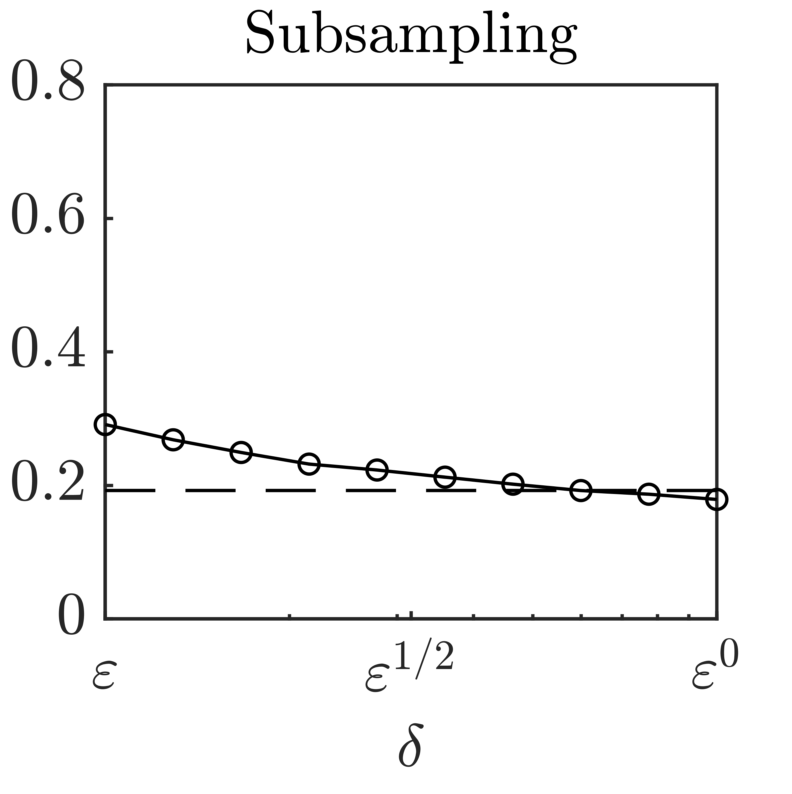
\includegraphics[]{Figures/OUSubs_s5} & 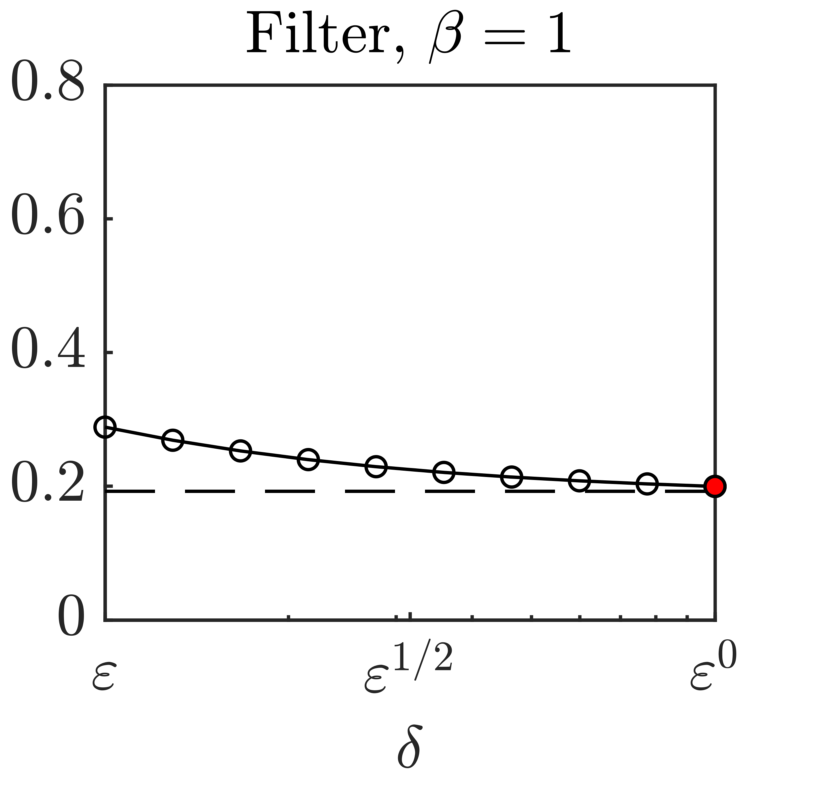
\includegraphics[]{Figures/OUFilt_s5_b1}  & 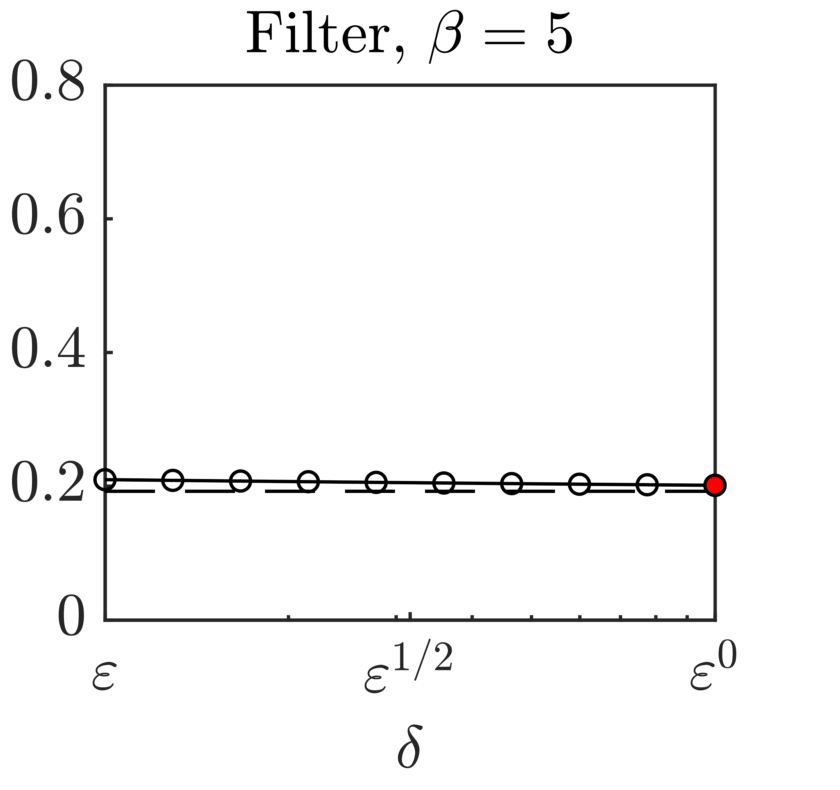
\includegraphics[]{Figures/OUFilt_s5_b5} \\ % & 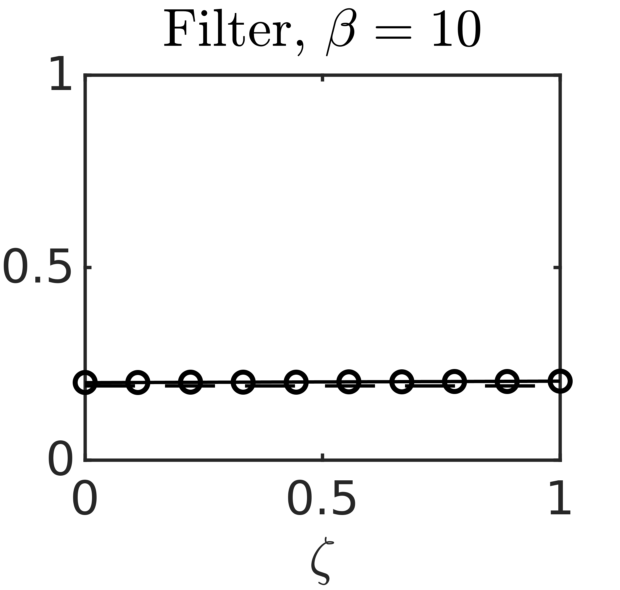
\includegraphics[]{Figures/OUFilt_s5_b10} \\
		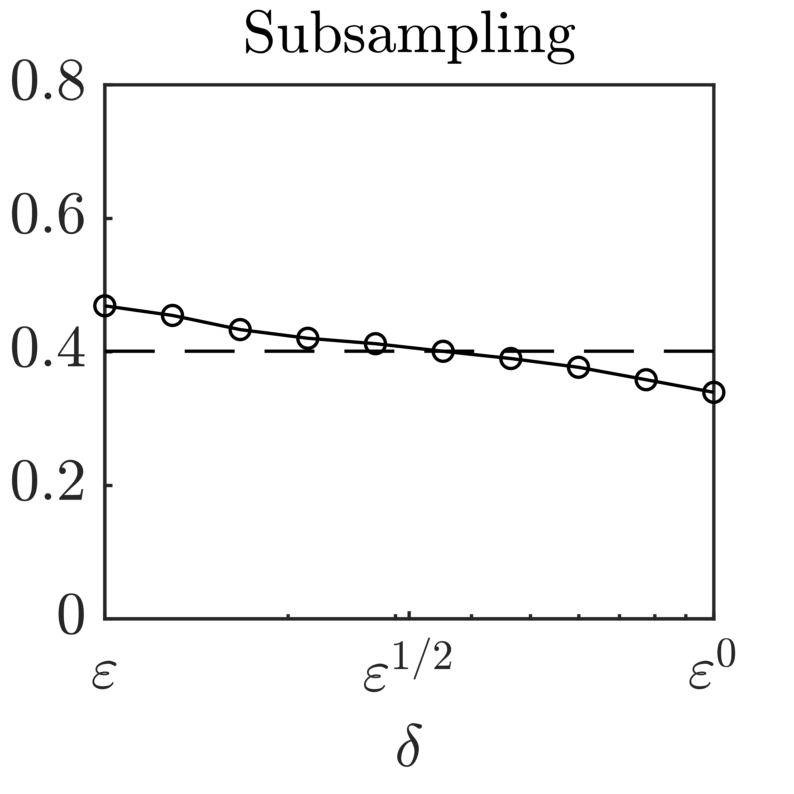
\includegraphics[]{Figures/OUSubs_s7} & 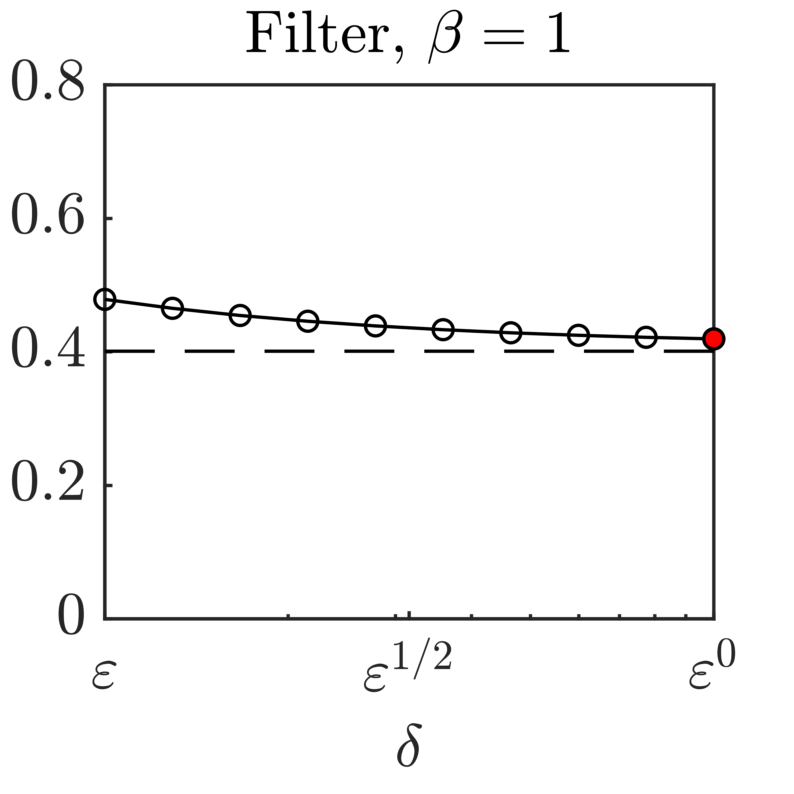
\includegraphics[]{Figures/OUFilt_s7_b1}  & 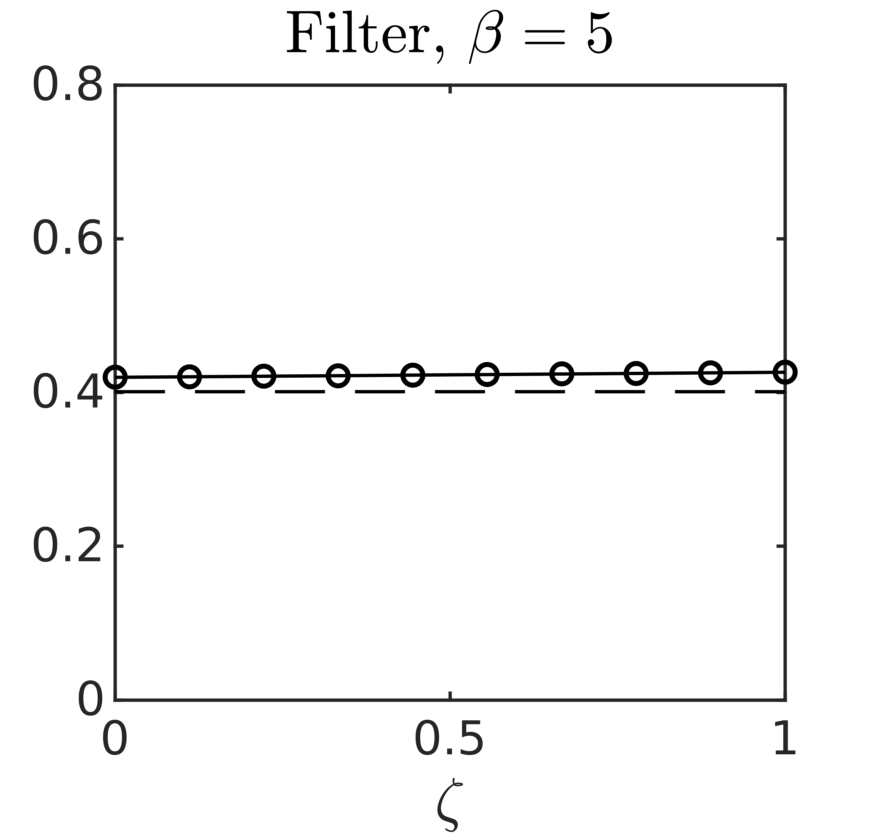
\includegraphics[]{Figures/OUFilt_s7_b5} \\ % & 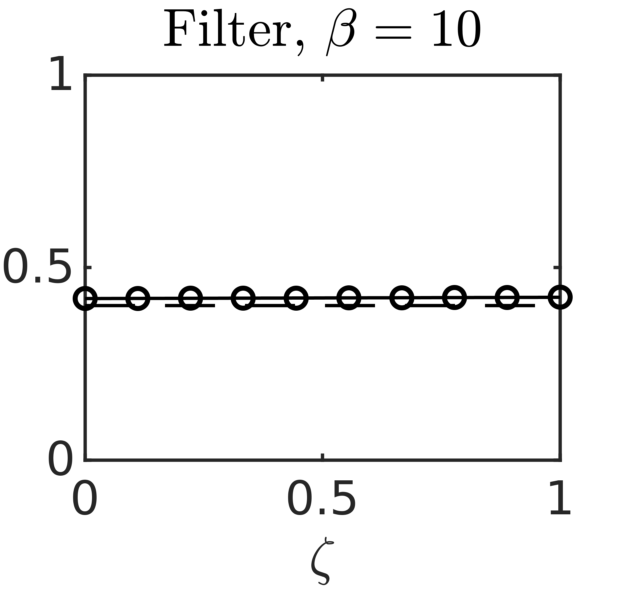
\includegraphics[]{Figures/OUFilt_s7_b10} \\
		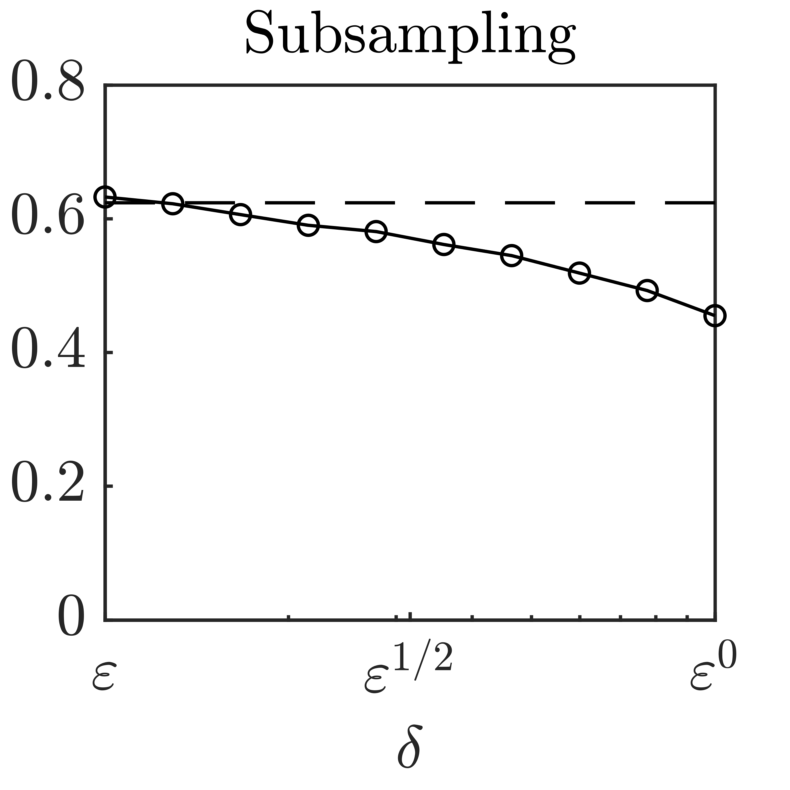
\includegraphics[]{Figures/OUSubs_s10} & 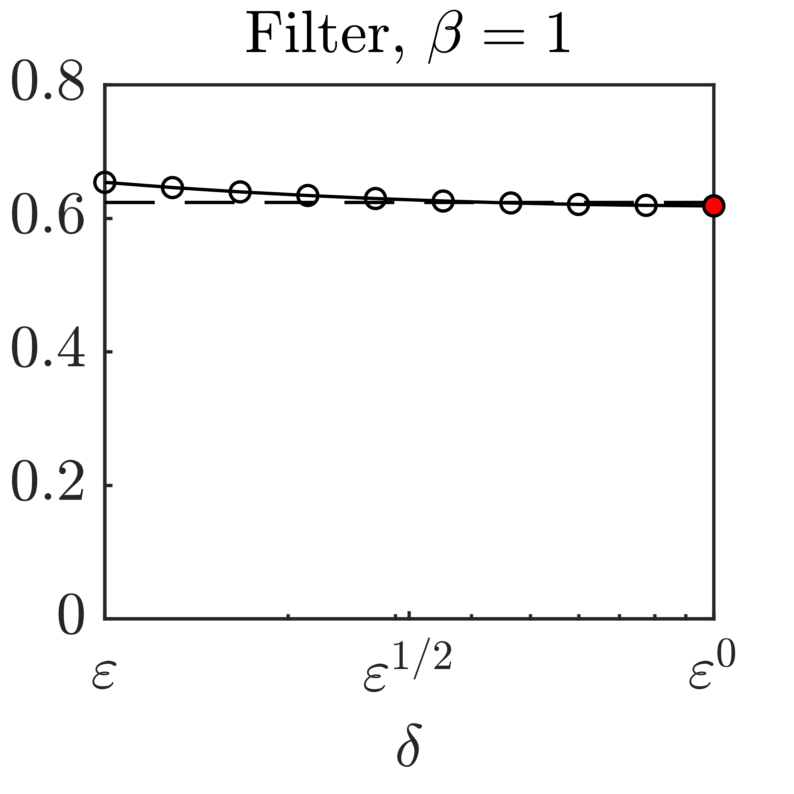
\includegraphics[]{Figures/OUFilt_s10_b1}  & 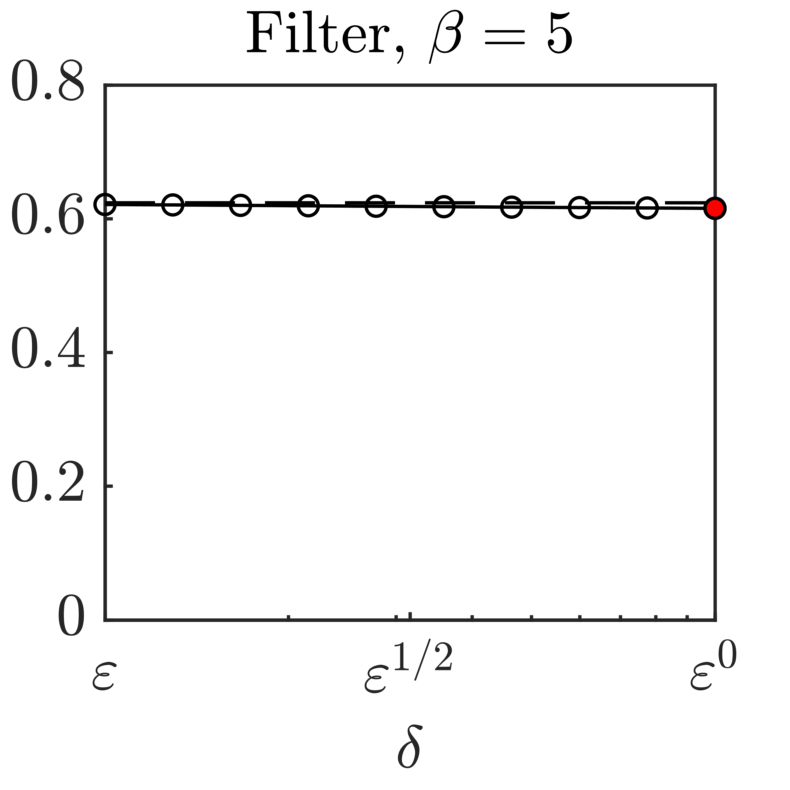
\includegraphics[]{Figures/OUFilt_s10_b5} % & 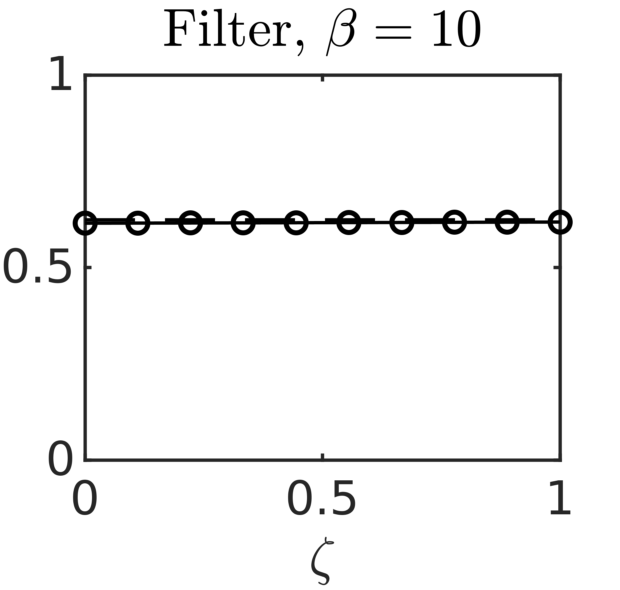
\includegraphics[]{Figures/OUFilt_s10_b10}
	\end{tabular}
	\caption{Results for the Ornstein--Uhlenbeck process. The axis of abscissae $\zeta$ represents the value of $\delta = \epl^\zeta$ for both subsampling and the filter. The three rows correspond to $\sigma = 0.5, 0.7, 1.0$ from top to bottom.}
	\label{fig:OU}
\end{figure}
We consider $N = 1$ and the quadratic potential $V(x) = x^2/2$. In this case, the solution of the homogenized equation is an Ornstein--Uhlenbeck process. Moreover, we set the multiscale equation \eqref{eq:SDE_MS} with $\epl = 0.1$ and the fast potential $p(y) = \cos(y)$. We generate data $X^\epl$ for $0 \leq t \leq T$ and $T = 10^3$ employing the Euler--Maruyama method with time step $\Delta_t = \epl^3$. 

As a first experiment, we consider the effect of setting different values of the parameter $\delta$ of the filter \eqref{eq:filter} on the estimator. As a comparison and for similarity with the subsampling approach, we consider $\delta = \epl^{\zeta}$ and vary $\zeta \in [0, 1]$. We employ the same values of $\delta$ for the subsampling, too, as the theoretical results guarantee convergence only for these values. Moreover, we repeat the experiments fixing $\beta = 1, 5$ and for three different values of the diffusion, i.e., we choose $\sigma = 0.5, 0.7, 1$. We report in Figure \ref{fig:OU} the experimental results. Let us remark that
\begin{enumerate}
	\item for $\sigma = 0.5$ the results given by subsampling and by the filter with $\beta = 1$ are similar, while for higher values of $\sigma$ the filtering approach seems better than subsampling, 
	\item in general, choosing a higher value of $\beta$ seems beneficial for the quality of the estimator,
	\item the dependence on $\delta$ of numerical results given by the filter seems relevant only in case $\beta = 1$ and for small values of $\sigma$. For $\beta = 1$ and higher values of $\sigma$, the estimator is stable with respect to this parameter, as predicted in Theorem \ref{thm:mainTheorem}. This can be observed for a higher value of $\beta$ but we have no theoretical guarantee in this case.
\end{enumerate}

As a second experiment, we therefore test the variability of the estimator with respect to $\beta$ in \eqref{eq:filter}. We repeat the numerical experiment in Figure \ref{fig:OU} and we choose to consider $\delta = \epl$, which corresponds to $\zeta = 1$ and seems to be the worst-case scenario for the filter, at least for $\beta = 1$. We consider again $\sigma = 0.5, 0.7, 1$ and vary $\beta = 1, 2, \ldots, 10$. Results, given in Figure \ref{fig:OUBeta}, show empirically that the estimator is fast stable with respect to $\beta$.

\begin{figure}[t]
	\centering
	\begin{tabular}{ccc}
		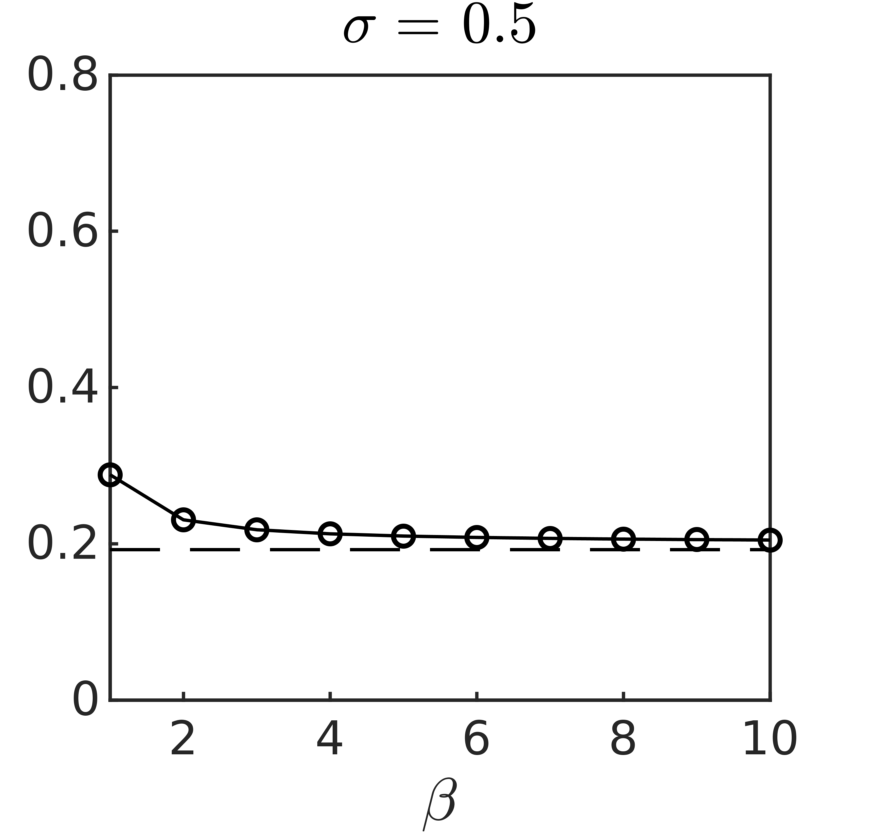
\includegraphics[]{Figures/OUBeta_s5} & 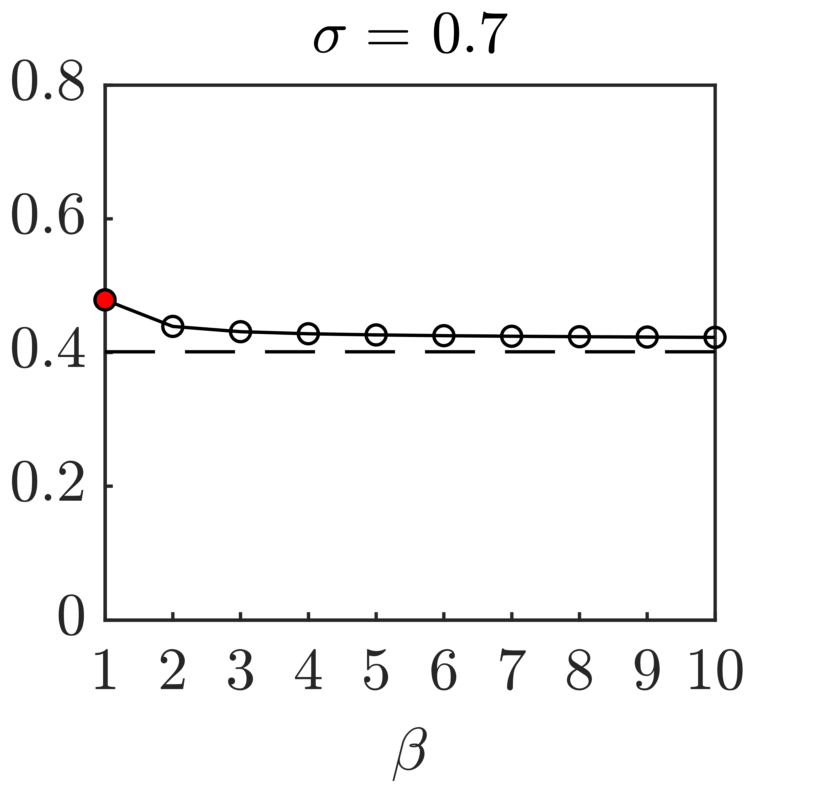
\includegraphics[]{Figures/OUBeta_s7}  & 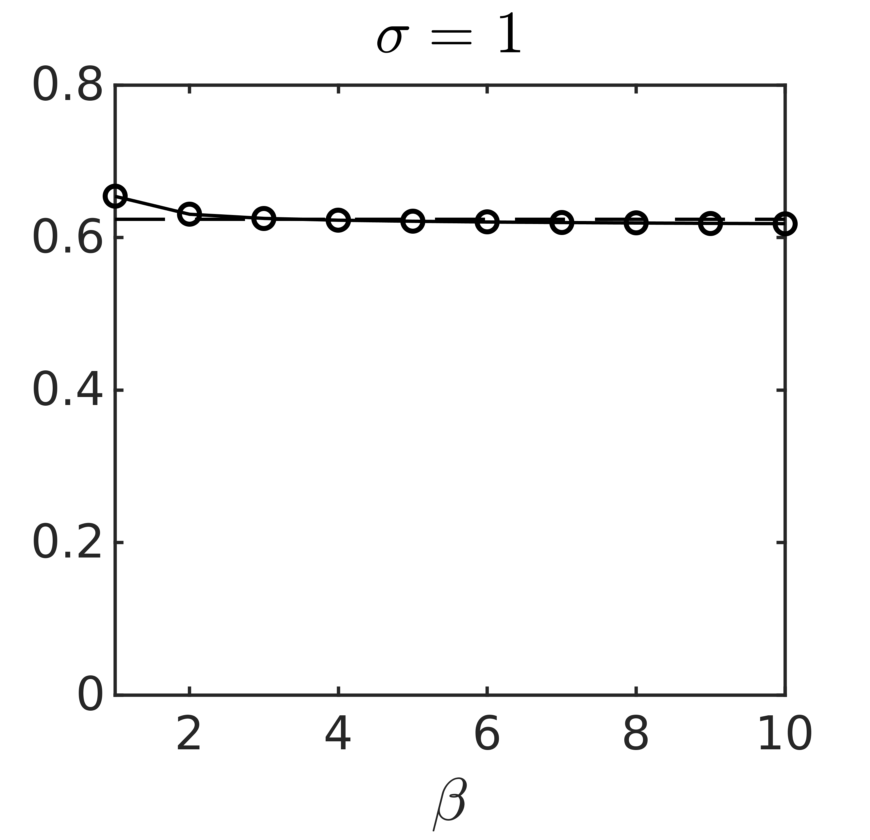
\includegraphics[]{Figures/OUBeta_s10} \\
	\end{tabular}
	\caption{Dependence of the estimator given by the filter for the Ornstein--Uhlenbeck process on the parameter $\beta$ in \eqref{eq:filter}. From left to right we consider different values of $\sigma$.}
	\label{fig:OUBeta}
\end{figure}

\subsection{Central limit theorem}
\begin{figure}[t]
	\centering
	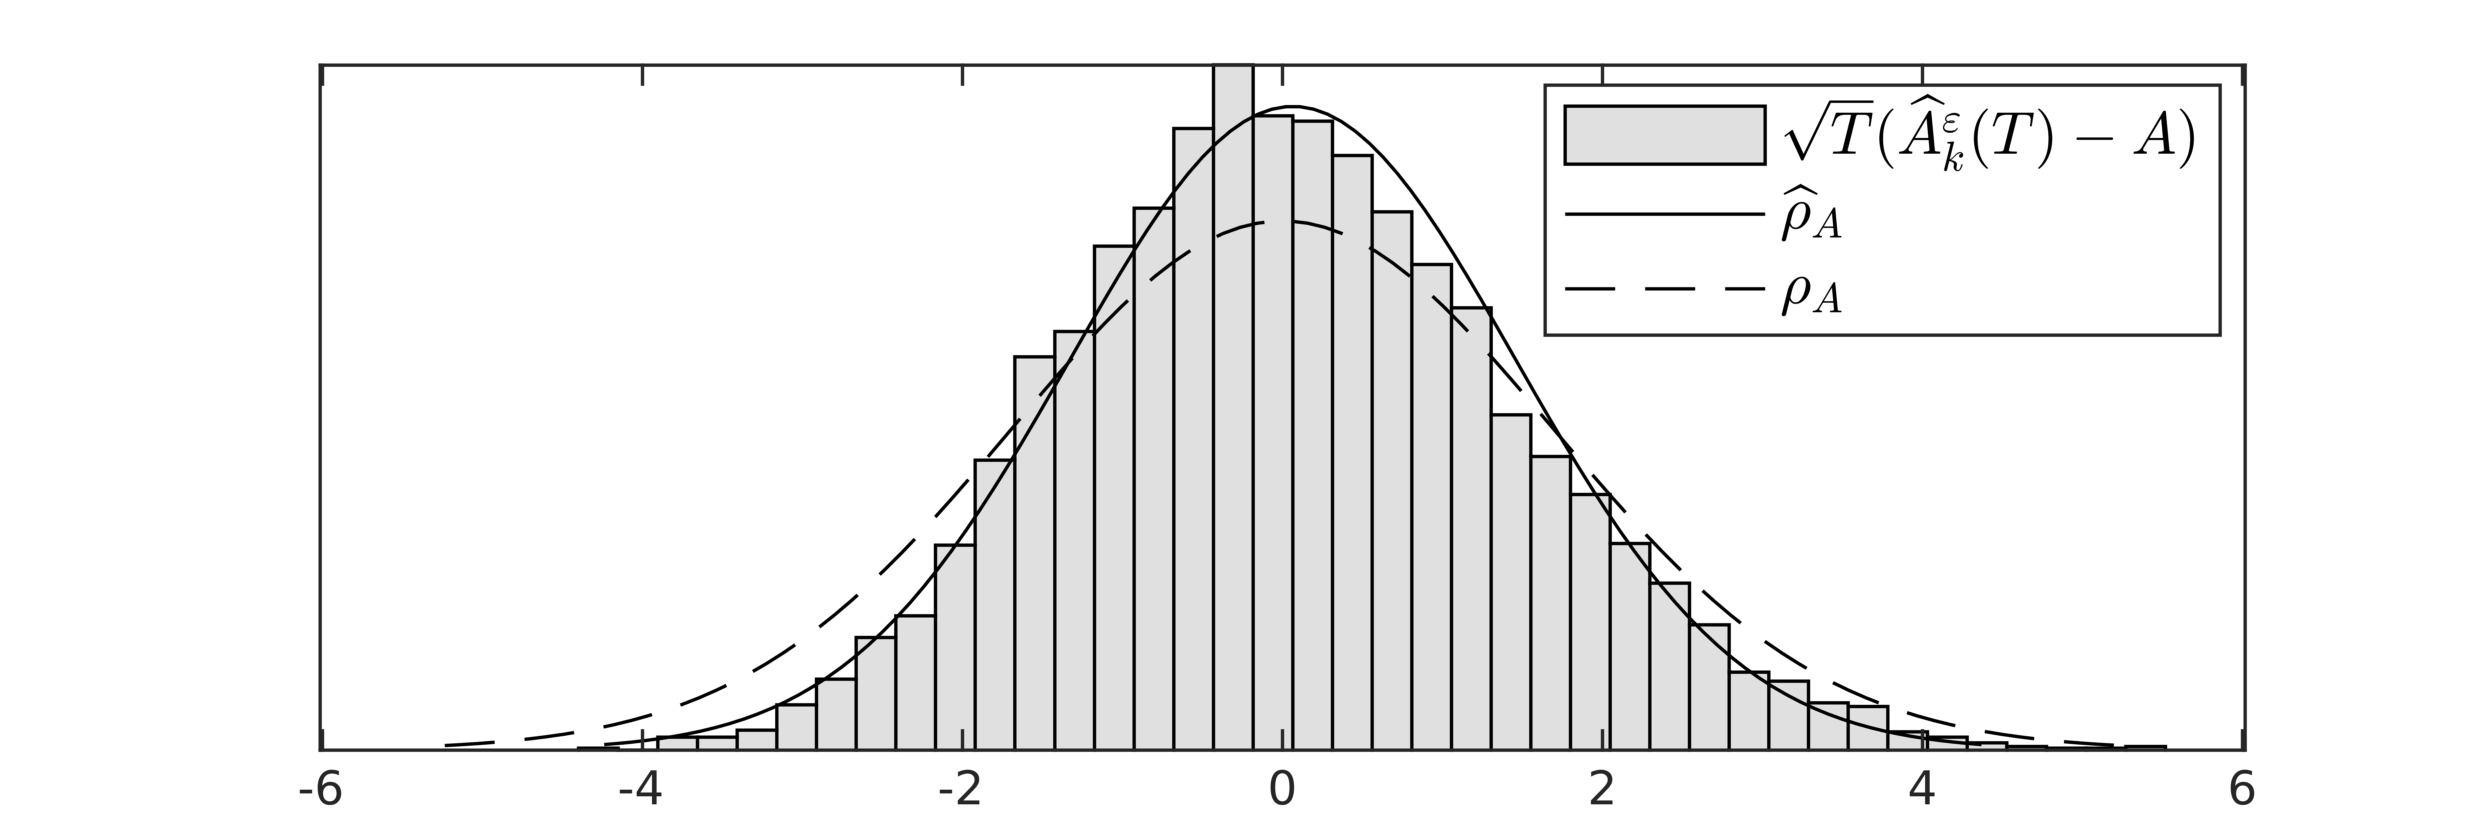
\includegraphics[]{Figures/CLT}
	\caption{Central limit theorem result. The histogram represents numerical results, the solid curve a Gaussian fit to the latter and the dashed curve the theoretical estimate given in Theorem \ref{thm:CLT}.}
	\label{fig:CLT}
\end{figure}

In this experiment we wish to confirm the validity of Theorem \ref{thm:CLT}. We consider the same test equation as for Section \ref{sec:Num_Param}, i.e., the quadratic potential $V(x) = x^2/2$ with fluctuating potential $p(y) = \sin(y)$, multiscale parameter $\epl = 0.05$ and diffusion coefficient $\sigma = 1$. The parameters of the filter are set to $\beta = 1$ and $\delta = 1$. We compute the estimator $\widehat A^\epl_k(T)$ with final time $T = 10^3$ on $2000$ realizations of the solution and estimate the quantity 
\begin{equation}	
	\Delta_A^\epl(T) \defeq \sqrt{T}\left(\widehat A^\epl_k(T) - A\right),	
\end{equation}
where $A$ is the drift coefficient of the homogenized equation. Results, depicted in Figure \ref{fig:CLT}, show that the distribution of $\Delta_A^\epl(T)$ indeed follows a zero-mean Gaussian law, \corr{whose covariance agrees with the theoretical results (?)}.

\subsection{Multi-dimensional drift coefficient}

\begin{figure}[t]
	\centering
	\begin{tabular}{ccc}
		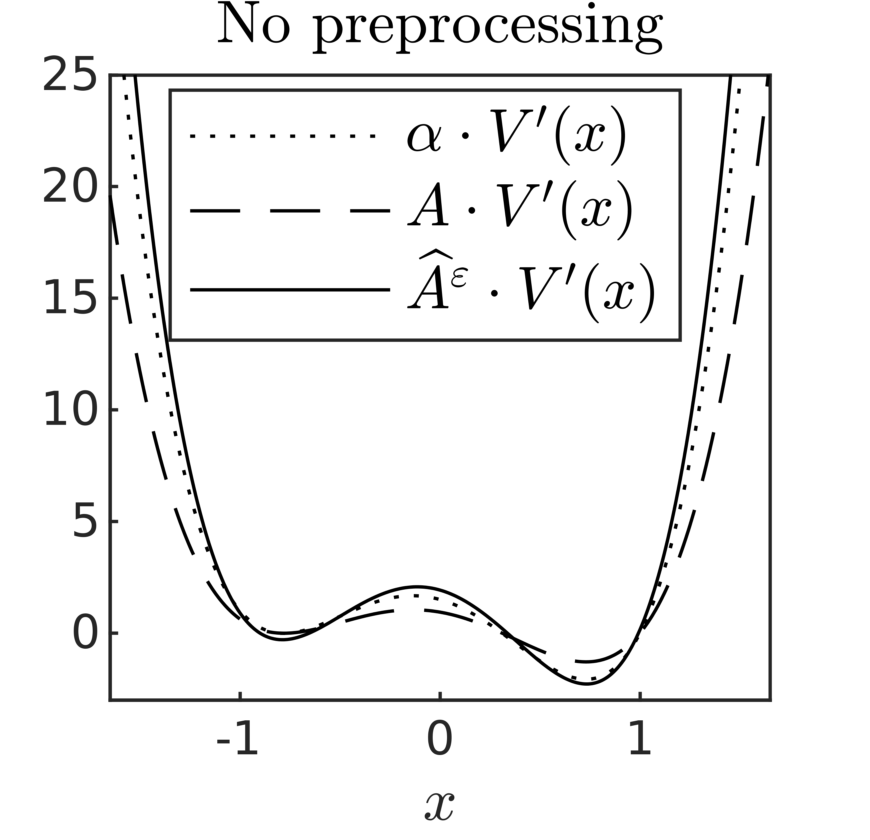
\includegraphics[]{Figures/KLNothing} & 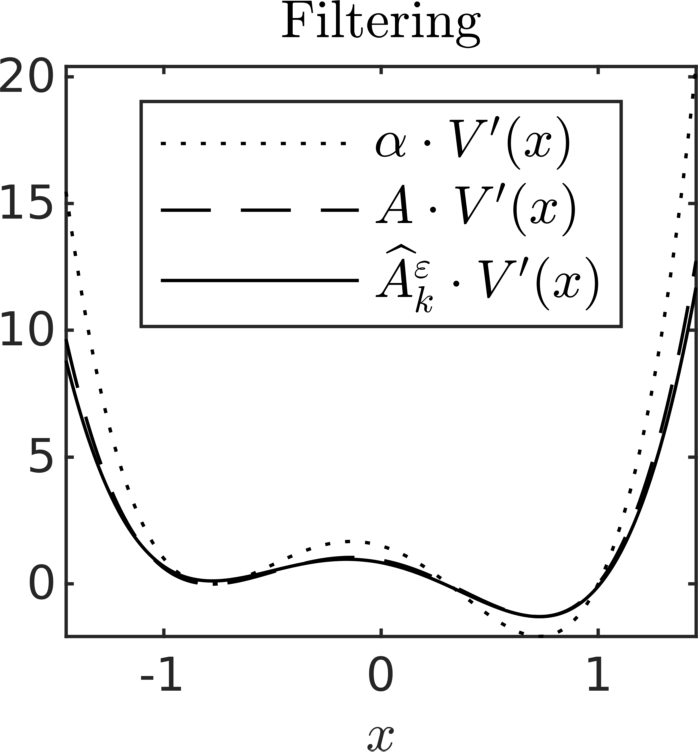
\includegraphics[]{Figures/KLFilt}  & 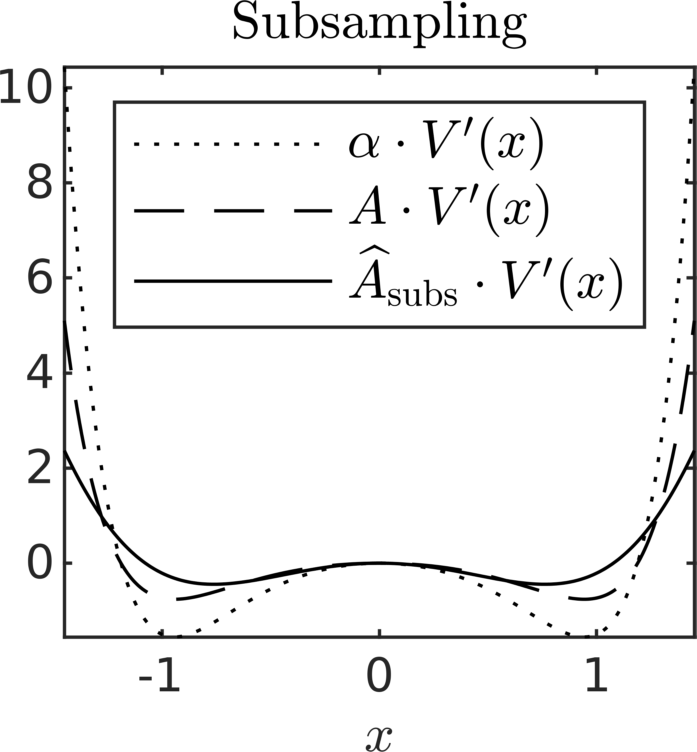
\includegraphics[]{Figures/KLSubs}
	\end{tabular}
	\caption{Results for the four-dimensional parameter. From left to right the potential function estimated with the data itself, the filter, subsampled data.}
	\label{fig:KLStyle}
\end{figure}

\begin{table}[t]
	\centering
	\begin{tabular}{cccccc}
		\toprule
		Coefficient & Multiscale & Homogenized & No preprocessing  & Filtering  		  & Subsampling  			 \\ 
		& $\alpha$ & $A$   & $\widehat A^\epl$ & $\widehat A^\epl_k$ & $\widehat A^\epl_\delta$ \\
		\midrule
		$1$ &-1   & -0.62 & -0.92 & -0.70 & -0.59\\
		$2$ &-0.5 & -0.31 & -0.70 & -0.27 & 0.05 \\
		$3$ & 0.5 & 0.31  & 0.55  & 0.31  & 0.14 \\
		$4$ & 1   & 0.62  & 1.22  & 0.57  & 0.13 \\
		\bottomrule
	\end{tabular}
	\caption{Numerical results for the four-dimensional parameter.}
	\label{tab:KLStyle}
\end{table}

Let us consider the Chebyshev polynomials of the first kind, i.e., the polynomials $T_i\colon \R \to \R$, $i=0, 1, \ldots$, defined by the recurrence relation
\begin{equation}
T_0(x) = 1, \quad T_1(x) = x, \quad T_{i+1}(x) = 2xT_i(x) - T_{i-1}(x).
\end{equation}
We consider the potential function $V(x)$ as in \eqref{eq:Potential} with
\begin{equation}
V_i(x) = T_i(x), \quad i =1, \ldots, 4.
\end{equation}
This potential function satisfies Assumption \ref{as:regularity} whenever $N$ is even and if the leading coefficient $\alpha_N$ is positive. We set $N = 4$ and the drift coefficient $\alpha = (-1, -1/2, 1/2, 1)$. With this drift coefficient, the potential function is of the bistable kind. Moreover, we set $\epl = 0.05$, the diffusion coefficient $\sigma = 1$, the fast potential $p(y) = \cos(y)$ and simulate a trajectory of $X^\epl$ for $0 \leq t \leq T$ with $T = 10^3$ employing the Euler--Maruyama method with time step $\Delta_t = \epl^3$. We estimate the drift coefficient $A \in \R^4$ with the estimators
\begin{enumerate}
	\item $\widehat A^\epl(T)$ based on the data $X^\epl$ itself,
	\item $\widehat A^\epl_\delta(T)$ based on subsampled data with subsampling parameter $\delta = \epl^{2/3}$,
	\item $\widehat A^\epl_k(T)$ based on filtered data $Z^\epl$ computed with $\beta = 1$ and $\delta = 1$.
\end{enumerate}
In particular, we pick this specific value of $\delta$ for the subsampling following the optimality criterion given in \cite{PaS07}. Results, given in Figure \ref{fig:KLStyle} and Table \ref{tab:KLStyle}, show that the filter-based estimation captures well the homogenized potential as well as the coefficient $A$. Moreover, it is possible to remark the negative result given by Theorem \ref{thm:Bias} holds in practice, i.e., with no pre-processing the estimator $\widehat A^\epl(T)$ tends to the drift coefficient $\alpha$ of the unhomogenized equation.

\subsection{The Bayesian approach: bistable potential}
\begin{figure}[t]
	\centering
	\begin{tabular}{ccc}
		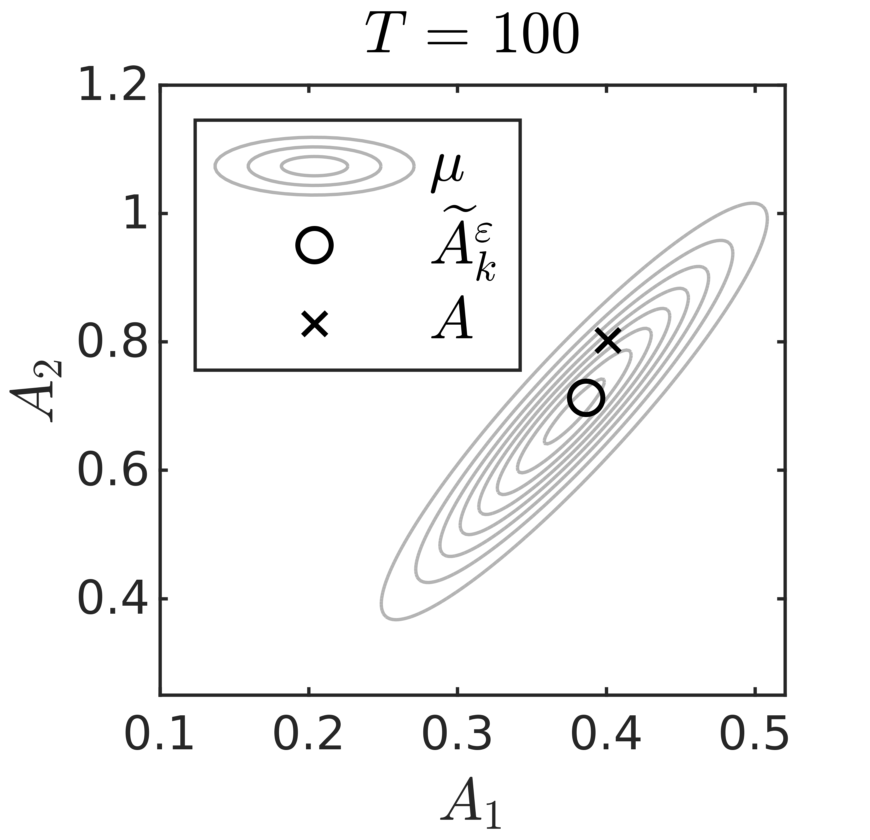
\includegraphics[]{Figures/Bayes_T100} & 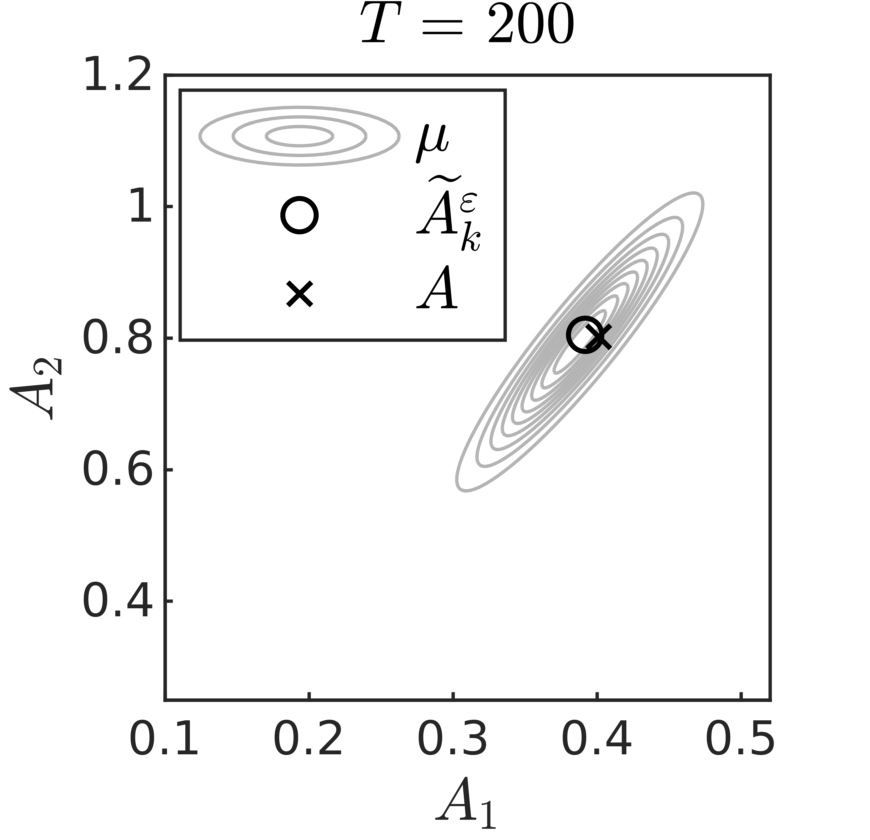
\includegraphics[]{Figures/Bayes_T200}  & 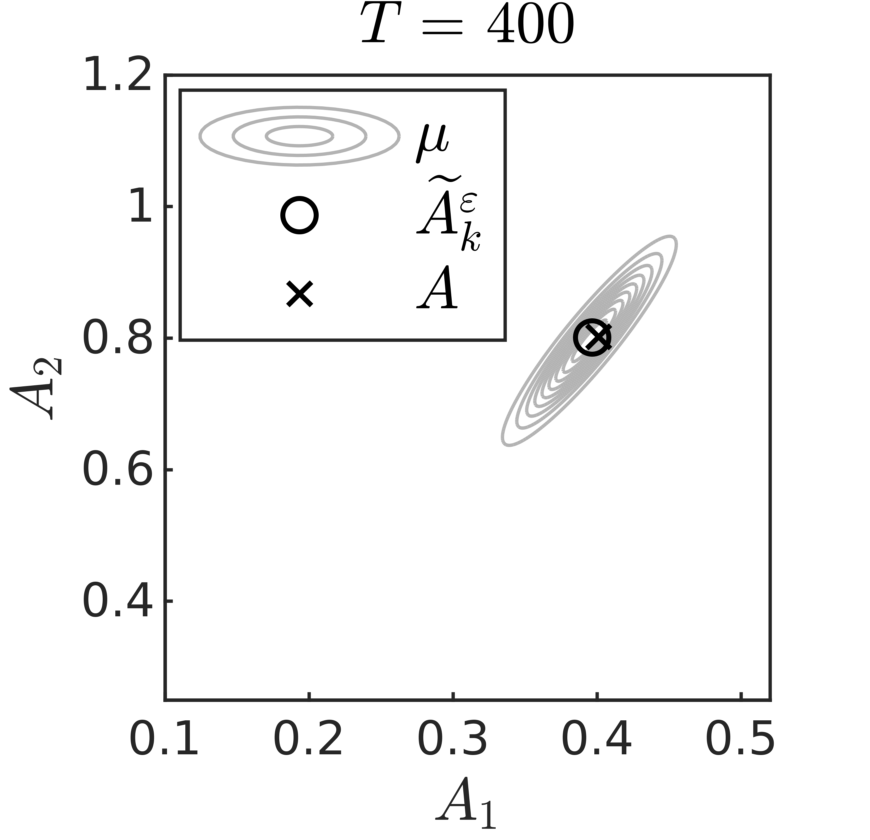
\includegraphics[]{Figures/Bayes_T400} \\
	\end{tabular}
	\caption{Posterior distributions over the parameter $A = (A_1, A_2)^\top$ for the bistable potential obtained with the filtering approach. The figures refer to final time $T = 100, 200, 400$ from left to right, respectively. The MLE $\widetilde A^\epl_k(t)$ is represented with a circle, while the true value $A$ of the drift coefficient of the homogenized equation is represented with a cross.}
	\label{fig:Bayes}
\end{figure}

In this numerical experiment we consider $N = 2$ and the bistable potential, i.e., the function $V$ defined as
\begin{equation}
	V(x) = \begin{pmatrix} \dfrac{x^4}{4} & -\dfrac{x^2}{2} \end{pmatrix}^\top,
\end{equation}
with coefficients $\alpha_1 = 1$ and $\alpha_2 = 2$. We then consider the multiscale equation with $\sigma = 0.7$, the fast potential $p(y) = \cos(y)$ and $\epl = 0.05$, thus simulating a trajectory $X^\epl$. We adopt here a Bayesian approach and compute the posterior distribution $\widetilde \mu_{T, \epl}$ obtained with the filtering approach introduced in Section \ref{sec:BayesianFilter}. The parameters of the filter are set to $\beta = 1$ and $\delta = \epl$ in \eqref{eq:filter}. Let us remark that in order to compute the posterior covariance the diffusion coefficient $\Sigma$ of the homogenized equation has to be known. In this case, we pre-compute the value of $\Sigma$ via the coefficient $K$ and the theory of homogenization, but let us remark that $\Sigma$ could be estimated employing the subsampling technique of \cite{PaS07}. We stop computations at times $T = 100, 200, 400$ in order to observe the shrinkage of the Gaussian posterior towards the MLE $\widetilde A^\epl_k(T)$ with respect to time. In Figure \ref{fig:Bayes}, we observe that the posterior does indeed shrink towards the MLE, which in turn gets progressively closer to the true value of the drift coefficient $A$ of the homogenized equation.

\section{Conclusion}

In this work we considered a novel methodology based on filtering for the estimation of the drift of multiscale diffusion processes. We proved results of ergodicity, convergence and, most importantly, unbiasedness of estimators drawn from our methodology. Moreover, we combined a Bayesian approach and our new technique to guarantee a robust uncertainty quantification of the inference procedure. Numerical experiments demonstrate how the filtering-based estimator requires less knowledge of the characteristic time-scales of the multiscale equation and how it can be employed as a black-box tool for parameter estimation on a range of academic examples. We believe this work gives way to several further developments. In particular, we believe it would be relevant to 
\begin{enumerate}
	\item analyse the filtering methodology for $\beta > 1$ in \eqref{eq:filter}, which seems to give more robust results in practice,
	\item extend the analysis to the non-parametric framework most likely by means of Bayesian regularization techniques,
	\item consider multiscale models for which the homogenized equation presents multiplicative noise,
	\item test the filtering methodology against real-world data,
	\item apply similar filtering methodologies to correct faulty behaviour of non likelihood-based estimators.
\end{enumerate} 

\begin{appendices}
	
\section{Proof of Lemmas}\label{ap:Proofs}

\begin{proof}[Proof of Lemma \ref{lem:density}] We have to show that the joint process solution to \eqref{eq:systemSDE} is hypo-elliptic. Denoting as $f\colon \R \to \R$ the function 
	\begin{equation}
	f(x) = -\alpha \cdot V'(x) - \frac1\epl p'\left(\frac{x}\epl\right),
	\end{equation}
	the generator of the process $(X^\epl, Z^\epl)^\top$ is given by
	\begin{equation}
	\mathcal L = f \partial_x + \sigma \partial_{xx}^2 + \frac1\delta (x - z)\partial_z \eqdef \mathcal X_0 + \sigma \mathcal X_1^2, 
	\end{equation}
	where 
	\begin{equation}
	\mathcal X_0 = f \partial_x + \frac1\delta (x - z)\partial_z, \quad \mathcal X_1 = \partial_x.
	\end{equation}
	The commutator $[\mathcal X_0, \mathcal X_1]$ applied to a test function $v$ then gives
	\begin{equation}
	\begin{aligned}
	[\mathcal X_0, \mathcal X_1]v &= f \partial_x^2 v + \frac1\delta (x - z) \partial_x \partial_z v  - \partial_x\left(f\partial_x v + \frac1\delta (x - z)\partial_z v\right)\\
	&= -\partial_x f \partial_x v - \frac1\delta \partial_z v.
	\end{aligned}
	\end{equation}
	Consequently, 
	\begin{equation}
	\mathrm{Lie}\left(\mathcal X_1, [\mathcal X_0, \mathcal X_1]\right) = \mathrm{Lie} \left(\partial_x, -\partial_x f \partial_x - \frac1\delta\partial_z\right),
	\end{equation}
	which spans the tangent space of $\R^2$ at $(x, z)$, denoted $T_{x, z}\R^2$. The desired result then follows from Hörmander's theorem (see e.g. \cite[Chapter 6]{Pav14}).
\end{proof}

\begin{proof}[Proof of Lemma \ref{lem:ergodicity}] Lemma \ref{lem:density} guarantees that the Fokker--Planck equation can be written directly from the system \eqref{eq:systemSDE}. For geometric ergodicity, let 
	\begin{equation}
	\mathcal S(x,z) \defeq \begin{pmatrix} -\alpha \cdot V'(x) - \frac1\epl p'(\frac{x}{\epl}) \\ \frac1\delta (x - z) \end{pmatrix} \cdot \begin{pmatrix} x \\ z \end{pmatrix} =  -\left(\alpha \cdot V'(x) + \frac1\epl p'\left(\frac{x}{\epl}\right)\right)x + \frac1\delta(xz-z^2).
	\end{equation}
	Due to Assumption \ref{as:regularity}\ref{as:regularity_diss}, Remark \ref{rem:regularity_diss} and Young's inequality, we then have for all $\gamma > 0$
	\begin{equation}
	\mathcal S(x,z) \leq a + \left(\frac{1}{2\gamma\delta} - b\right)x^2 + \frac1\delta\left(\frac{\gamma}{2} - 1\right)z^2.
	\end{equation}
	We choose $\gamma = \gamma^* \defeq 1 - b\delta + \sqrt{1 + (1 - b\delta)^2} > 0$ so that
	\begin{equation}
	C(\gamma^*) \defeq -\frac{1}{2\gamma^*\delta} + b = -\frac1\delta\left(\frac{\gamma^*}{2} - 1\right),
	\end{equation}
	and we notice that $C(\gamma^*) > 0$ if $\delta > 1/(4b)$. In this case, we have
	\begin{equation}
	\mathcal S(x, z) \leq a - C(\gamma^*) \norm{\begin{pmatrix} x & z \end{pmatrix}^\top}^2,
	\end{equation}
	and problem \eqref{eq:systemSDE} is dissipative. The result then follows from \cite[Theorem 4.4]{MSH02}.
\end{proof}

\begin{proof}[Proof of Lemma \ref{lem:FPMarginal}] Integrating equation \eqref{eq:FPsystem} with respect to $z$ we obtain the stationary Fokker--Planck equation for the process $X^\epl$, i.e.
	\begin{equation}
	\label{FPx}
	\sigma (\phi^\epl)''(x) + \frac{\d}{\d x} \left( \left ( \alpha \cdot V'(x) + \frac{1}{\epl} p' \left ( \frac{x}\epl \right ) \right ) \phi^\epl(x)\right) = 0,
	\end{equation}
	whose solution is given by
	\begin{equation}
	\phi^\epl(x) = \frac{1}{C_{\phi^\epl}} \exp\left(- \frac{1}{\sigma} \alpha \cdot V(x) - \frac{1}{\sigma} p \left ( \frac{x}\epl \right )\right),
	\end{equation}
	and which proves \eqref{eq:marginalX}. By integrating equation \eqref{eq:FPsystem} with respect to $x$ and integrating by parts we obtain
	\begin{equation}
	\psi^\epl(z) + z (\psi^\epl)'(z) = \frac{\d}{\d z} \int_{\R} x \rho^\epl(x,z) \dd x,
	\end{equation}
	which can be written as
	\begin{equation}
	\frac{\d}{\d z} (z \psi^\epl(z)) = \frac{\d}{\d z} \int_{\R} x \rho^\epl(x,z) \dd x.
	\end{equation}
	Now, since $\psi^\epl$ is the density of a probability distribution, this implies that 
	\begin{equation}\label{FPz}
	z \psi^\epl(z) = \int_{\R} x \rho^\epl(x,z) \dd x,
	\end{equation}
	which, replacing the decomposition \eqref{eq:densityDecomposition}, yields
	\begin{equation} \label{eq:z_condition}
	z = \int_{\R} x \phi^\epl(x) R^\epl(x,z) \dd x.
	\end{equation}
	In view of \eqref{eq:densityDecomposition} and \eqref{FPx}, equation \eqref{eq:FPsystem} can be rewritten as
	\begin{equation}\label{eq:psiEqualityPDE}
	\sigma \phi^\epl \psi^\epl \partial^2_{xx} R^\epl + \frac{1}{\delta} \phi^\epl \psi^\epl R^\epl + \sigma (\phi^\epl)' \psi^\epl \partial_x R^\epl + \frac{1}{\delta} (z-x) \phi^\epl ((\psi^\epl)' R + \psi^\epl \partial_z R^\epl) = 0.
	\end{equation}
	We now multiply the equation above by $x$ and integrate with respect to $x$. Let us consider some simplifications explicitly. First, an integration by parts yields
	\begin{equation}\label{eq:psiEqualityPDE_1}
	\begin{aligned}
	\sigma \psi^\epl \int_{\R}  x \phi^\epl \partial^2_{xx} R^\epl \dd x+ \sigma \psi^\epl \int_{\R} x (\phi^\epl)' \partial_x R^\epl \dd x &= -\sigma \psi^\epl \int_{\R} \phi^\epl \partial_x R^\epl \dd x.
	\end{aligned}
	\end{equation}
	Then, applying \eqref{eq:z_condition}, we have
	\begin{equation}\label{eq:psiEqualityPDE_2}
	\frac1\delta \psi^\epl \int_{\R} x \phi^\epl  R^\epl \dd x = \frac1\delta z \psi^\epl.
	\end{equation}
	Moreover, again applying \eqref{eq:z_condition}, we can compute
	\begin{equation}\label{eq:psiEqualityPDE_3}
	\begin{aligned}
	\frac1\delta (\psi^\epl)' \int_\R (z-x)x \phi^\epl  R \dd x = \frac1\delta (\psi^\epl)' \left(z^2 - \int_{\R} x^2 \phi^\epl R^\epl \dd x\right).
	\end{aligned}
	\end{equation}
	Finally, we compute the last term always applying \eqref{eq:z_condition} obtaining
	\begin{equation}\label{eq:psiEqualityPDE_4}
	\frac1\delta \psi^\epl \int_\R (z-x)x \phi^\epl \partial_z R \dd x = \frac1\delta \psi^\epl\left(z - \int_{\R} x^2 \phi^\epl \partial_z R^\epl \dd x\right).
	\end{equation}
	Replacing the equalities \eqref{eq:psiEqualityPDE_1}, \eqref{eq:psiEqualityPDE_2}, \eqref{eq:psiEqualityPDE_3} and \eqref{eq:psiEqualityPDE_4} into \eqref{eq:psiEqualityPDE} we obtain
	\begin{equation}
	(\psi^\epl)' \left ( z^2 - \int_{\R} x^2 \phi^\epl R^\epl \dd x \right ) + \psi^\epl \left ( 2z - \int_{\R} x^2 \phi^\epl \partial_z R^\epl \dd x - \delta \sigma \int_{\R} \phi^\epl \partial_x R^\epl \dd x \right ) = 0.
	\end{equation}
	We rewrite the equality above as
	\begin{equation} \label{eq:psiEquality}
	\delta \sigma \psi^\epl(z) \int_{\R} \phi^\epl(x) \partial_x R^\epl(x, z) \dd x = 
	\begin{aligned}[t] &(\psi^\epl)'(z) z^2 - (\psi^\epl)'(z) \int_{\R} x^2 \phi^\epl(x) R^\epl(x, z) \dd x \\
	& + 2 \psi^\epl(x) z - \psi^\epl \int_{\R} x^2 \phi^\epl(x) \partial_z R^\epl(x, z) \dd x.
	\end{aligned}
	\end{equation}
	Multiplying by $V'(z)$, integrating with respect to $z$ and integrating by parts, we obtain the following identity in $\R^N$
	\begin{equation}
	\begin{aligned}
	\sigma \delta \int_{\R} \int_{\R} V'(z) \phi^\epl(x) \psi^\epl(z) \partial_x R^\epl(x,z) \dd x \dd z &=  \int_{\R} \int_{\R} (x^2 - z^2) V''(z) \rho_\epl(x,z) \dd x \dd z \\
	&= \E^{\rho^\epl}[((X^\epl)^2 - (Z^\epl)^2)V''(Z^\epl)],
	\end{aligned}
	\end{equation}
	which is the desired result.
\end{proof}

\begin{proof}[Proof of Lemma \ref{lem:convMeasure}] Let $(X, Z)^\top \defeq \left((X_t, Z_t)^\top, 0\leq t \leq T\right)$ be the solution of
	\begin{equation}
	\label{eq:systemSDEHom}
	\begin{aligned}
	\d X_t &= -A \cdot V'(X_t) \dd t + \sqrt{2\Sigma} \dd W_t, \\
	\d Z_t &= \frac{1}{\delta} \left ( X_t - Z_t \right ) \dd t,
	\end{aligned}
	\end{equation} 
	with $(X_0, Z_0)^\top \sim \mu^0$. The arguments of Section \ref{sec:ergodic} can be repeated to conclude that the invariant measure of $(X, Z)^\top$ admits a smooth density $\rho^0$ which satisfies \eqref{eq:FPsystem_homogenized}. Moreover, standard homogenization theory (see e.g. \cite[Chapter 3]{BLP78}) guarantees that $(X^\epl,Z^\epl)^\top \to (X,Z)^\top$ for $\epl \to 0$ in law as random variables with values in $\mathcal C^0([0, T]; \R^2)$. The Portmanteau theorem can be employed to conclude that the measure $\mu^\epl$ converges weakly to $\mu^0$ for $\epl \to 0$.
\end{proof}

\section{Proof of Theorem \ref{thm:CLT}}\label{ap:CLT}

Let us first introduce a technical Lemma.
\begin{lemma}\label{lem:CLT} Let $\mathcal L_\epl$ be the generator of the couple $(X^\epl, Z^\epl)^\top$, i.e.,
	\begin{equation}
		\mathcal L_\epl = -\left(\alpha \cdot V'(x) + \frac1\epl p'\left(\frac{x}{\epl}\right)\right)\partial_x + \frac1\delta (x - z) \partial_z  + \sigma \partial^2_{xx}.
	\end{equation} 
	Moreover, let $\rho^\epl$ be the invariant measure of $(X^\epl, Z^\epl)^\top$ and $\Phi^\epl\colon \R^2 \to \R^N$ be the solution of 
	\begin{equation}\label{eq:CLT_Poisson}
		-\mathcal L_\epl \Phi^\epl = \chi -  \E^{\rho^\epl}[\chi(X^\epl, Z^\epl)],
	\end{equation}
	for $\chi \colon \R^2 \to \R^N$ satisfying $\E^{\rho^\epl}[\Phi^\epl(X^\epl, Z^\epl)] = 0$. Then, it holds
	\begin{equation}\label{eq:CLT_PoissonIto}
		\frac{1}{T} \int_0^T  \chi(X_t^\epl, Z_t^\epl) \dd t = \E^{\rho^\epl}[\chi(X^\epl, Z^\epl)] - \frac{R^\epl(T)}{T} + \sqrt{2\sigma}\frac{S^\epl(T)}{T},
	\end{equation}
	where
	\begin{equation}\label{eq:CLT_PoissonRemainders}
		R^\epl(T) \defeq \Phi^\epl(X^\epl_T, Z^\epl_T) - \Phi^\epl(X^\epl_0, Z^\epl_0), \quad S^\epl(T) \defeq \int_0^T \partial_x \Phi^\epl(X_t^\epl, Z_t^\epl) \dd W_t.
	\end{equation}
	Moreover, it holds
	\begin{equation}\label{eq:CLT_Equiv}
		2\sigma \E^{\rho^\epl}[\partial_x \Phi^\epl(X^\epl, Z^\epl) \otimes \partial_x \Phi^\epl(X^\epl, Z^\epl)] = \E^{\rho^\epl}
		\begin{aligned}[t]
		[&\chi(X^\epl, Z^\epl) \otimes \Phi^\epl(X^\epl, Z^\epl) \\
		&+ \Phi^\epl(X^\epl, Z^\epl) \otimes \chi(X^\epl, Z^\epl)].
		\end{aligned}
	\end{equation}	
\end{lemma}
\begin{proof} The proof of \eqref{eq:CLT_PoissonIto} and \eqref{eq:CLT_PoissonRemainders} is an application of the Itô formula (see e.g. \cite[Remark 6.17]{PaS08}). For \eqref{eq:CLT_Equiv}, it is possible to show that since $\mathcal L_\epl^*\rho^\epl = 0$ it holds 
	\begin{equation}
		\mathcal L_\epl^* (\Phi^\epl \rho) = 2 \sigma \rho^\epl \partial_{xx}^2 \Phi^\epl - \rho^\epl \mathcal L_\epl\Phi^\epl + 2 \sigma \partial_x \Phi^\epl \partial_x \rho^\epl.
	\end{equation}
	Therefore, an integration by parts yields 
	\begin{equation}
	\begin{aligned}
		\E^{\rho^\epl}[\mathcal L_\epl \Phi^\epl(X^\epl, Z^\epl) \otimes \Phi^\epl(X^\epl, Z^\epl)] &= 	\int_{\R}\int_{\R} \Phi^\epl \otimes \mathcal L_\epl^*\left(\Phi^\epl \rho^\epl\right) \dd x \dd z \\
		&= -\int_{\R}\int_{\R}\Phi^\epl \otimes \mathcal L_\epl \Phi^\epl \rho^\epl \dd x \dd z- 2\sigma \int_{\R}\int_{\R} \partial_x \Phi^\epl \otimes \partial_x \Phi^\epl \rho^\epl \dd x \dd z\\
		&= 
		\begin{aligned}[t]
		&-\E^{\rho^\epl}[\Phi^\epl(X^\epl, Z^\epl) \otimes \mathcal L_\epl \Phi^\epl(X^\epl, Z^\epl)] \\
		&- 2\sigma \E^{\rho^\epl}[\partial_x \Phi^\epl(X^\epl, Z^\epl) \otimes \partial_x \Phi^\epl(X^\epl, Z^\epl)].
		\end{aligned}
	\end{aligned}
	\end{equation}
	Finally, since $\E^{\rho^\epl}[\Phi(X^\epl, Z^\epl)] = 0$ 
	\begin{equation}
	\begin{aligned}
		2\sigma \E^{\rho^\epl}[\partial_x \Phi^\epl(X^\epl, Z^\epl) \otimes \partial_x \Phi^\epl(X^\epl, Z^\epl)] &= -\E^{\rho^\epl}
		\begin{aligned}[t]
		[&\mathcal L_\epl \Phi^\epl(X^\epl, Z^\epl) \otimes \Phi^\epl(X^\epl, Z^\epl) \\
		& + \Phi^\epl(X^\epl, Z^\epl) \otimes \mathcal L_\epl \Phi^\epl(X^\epl, Z^\epl)]
		\end{aligned}
		\\
		&= \E^{\rho^\epl}
		\begin{aligned}[t]
		[&\chi(X^\epl, Z^\epl) \otimes \Phi^\epl(X^\epl, Z^\epl) \\
		&+ \Phi^\epl(X^\epl, Z^\epl) \otimes \chi(X^\epl, Z^\epl)],
		\end{aligned}
	\end{aligned}
	\end{equation}
	which is the desired result.
\end{proof}

We can now proceed with the main proof.
\begin{proof}[Proof of Theorem \ref{thm:CLT}] Let us introduce the notation
	\begin{equation}\label{eq:CLT_DefMEps}
	\mathcal M_\epl \defeq \E^{\rho^\epl} [ V'(Z^\epl) \otimes V'(X^\epl) ], \quad \mathcal M_0 \defeq \E^{\rho^0} [ V'(Z) \otimes V'(X) ],
	\end{equation}
	and the notation
	\begin{equation}
	\mathfrak p_\epl \defeq \E^{\rho^\epl} \left [ \frac{1}{\epl} p' \left ( \frac{X^\epl}{\epl} \right ) V'(Z^\epl) \right ]\
	\end{equation}
	and let us remark that from the proof of Theorem \ref{thm:mainTheorem} one can deduce the equalities
	\begin{equation}\label{eq:CTL_A}
	A = \frac1\delta \mathcal M_0^{-1} \E^{\rho^0}[(X^2 - Z^2)V''(Z)],
	\end{equation}
	and
	\begin{equation}\label{eq:CTL_alpha}
	\alpha = \mathcal M_\epl^{-1} \left(\frac1\delta \E^{\rho^\epl}[((X^\epl)^2 - (Z^\epl)^2)V''(Z^\epl)] - \mathfrak p_\epl \right).
	\end{equation}
	Let us furthermore remark that the decomposition \eqref{eq:alphaDecomposition} yields
	\begin{equation}
	\sqrt{T}\left(\widehat A^\epl_k(T) - A\right) = \sqrt{T} \left(\alpha - A + I_1^\epl - I_2^\epl\right).
	\end{equation}
	Replacing the expression for $A$ and $\alpha$ given in \eqref{eq:CTL_A} and \eqref{eq:CTL_alpha}, we get
	\begin{equation}
	\begin{aligned}
	\sqrt{T}\left(\widehat A^\epl_k(T) - A\right) &= \sqrt{T}\left( I_1^\epl(T) - \mathcal M_\epl^{-1} \mathfrak p_\epl \right) \\
	&+  \frac{\sqrt{T}}\delta \left( \mathcal M_\epl^{-1} \E^{\rho^\epl}[((X^\epl)^2 - (Z^\epl)^2)V''(Z^\epl)] - \mathcal M_0^{-1} \E^{\rho^0}[(X^2 - Z^2)V''(Z)] \right) \\
	&- \sqrt{T} I_2^\epl(T).
	\end{aligned}
	\end{equation}
	\corr{Third term is OK:} We rewrite the term involving $I_2^\epl(T)$ as
	\begin{equation}
	\sqrt{T} I_2^\epl(T) = \frac{\sqrt{2\sigma}}{\sqrt{T}} \widetilde M^{-1} Q^\epl(T),
	\end{equation}
	where, since $Z_t^\epl$ is adapted with respect to the natural filtration $\mathcal F_t$ of the Wiener process $W \defeq \left(W_t, t \geq 0\right)$, the quantity
	\begin{equation}
	Q^\epl(T) \defeq \int_0^T V'(Z^\epl_t) \dd W_t,
	\end{equation}
	is a martingale whose quadratic variation is given by
	\begin{equation}
	\langle Q^\epl \rangle_T = \int_0^T V'(Z^\epl_t) \otimes V'(Z^\epl_t) \dd t. 
	\end{equation}
	Since the ergodic theorem guarantees that 
	\begin{equation}
	\lim_{T\to\infty}\frac{\langle Q^\epl \rangle_T}{T} = \E^{\rho^\epl}[V'(Z^\epl) \otimes V'(Z^\epl)], \quad \text{in } L^1(\mu^\epl),
	\end{equation}
	the martingale central limit theorem gives 
	\begin{equation}
	\lim_{T\to\infty}\frac{1}{\sqrt{T}} Q^\epl(T) = \Xi^\epl, \quad \text{in law},
	\end{equation}
	where $\Xi^\epl \sim \mathcal N(0, \E^{\rho^\epl}[V'(Z^\epl) \otimes V'(Z^\epl)])$.
	Now, by the ergodic theorem 
	\begin{equation}
	\lim_{T \to \infty} \widetilde M^{-1} = \mathcal M_\epl^{-1}, \quad \text{a.s.}
	\end{equation}
	Therefore, we have by Slutsky's theorem that
	\begin{equation}
	\lim_{T \to \infty} \sqrt{T} I_2^\epl(T) = \Lambda^\epl \sim \mathcal N\left(0, \Gamma^\epl\right), \quad \text{in law}.
	\end{equation}
	where the covariance matrix $\Gamma^\epl$ is given by
	\begin{equation}
	\Gamma^\epl = 2\sigma \mathcal M_\epl^{-1}\E^{\rho^\epl}[V'(Z^\epl) \otimes V'(Z^\epl)]\mathcal M_\epl^{-\top}.
	\end{equation}
	Finally, we denote by $\Lambda$ the limit for $\epl \to 0$ of the sequence of Gaussian random variables $\Lambda^\epl$.
	
	\corr{Idea for the first term:} Let us introduce the notation
	\begin{equation}
	J_1^\epl(T) \defeq \sqrt{T}\left( I_1^\epl(T) - \mathcal M_\epl^{-1} \mathfrak p_\epl\right),
	\end{equation}
	and let us remark that we can rewrite
	\begin{equation} \label{eq:decomposition_first_term}
	\begin{aligned}
	J_1^\epl(T) &= \sqrt{T} \left(\frac1T \int_0^T V'(Z^\epl_t) \otimes V'(X^\epl_t) \dd t\right)^{-1}\left(\frac1T \int_0^T \frac{1}{\epl} p' \left ( \frac{X^\epl_t}{\epl} \right ) V'(Z^\epl_t) \dd t - \mathfrak p_\epl \right) \\
	& \quad + \sqrt{T} \left(\left(\frac1T \int_0^T V'(Z^\epl_t) \otimes V'(X^\epl_t) \dd t\right)^{-1} - \mathcal M_\epl^{-1}\right) \mathfrak p_\epl\\
	&\eqdef J_{1,1}^\epl(T) + J_{1,2}^\epl(T).
	\end{aligned}
	\end{equation}
	Let us denote by $\Phi_1^\epl$ the solution of \eqref{eq:CLT_Poisson} in Lemma \ref{lem:CLT} with right hand side
	\begin{equation}
	\chi_1(x, z) = \frac 1 \epl p' \left ( \frac x \epl \right ) V'(z).
	\end{equation}
	Then, denoting as $R_1^\epl(T)$ and $S_1^\epl(T)$ the quantities introduced in \eqref{eq:CLT_PoissonRemainders} with $\Phi_1^\epl$ in place of $\Phi^\epl$, we have
	\begin{equation}
	J_{1,1}^\epl(T)= \sqrt{T} \left(\frac1T \int_0^T V'(Z^\epl_t) \otimes V'(X^\epl_t) \dd t\right)^{-1} \left( -\frac{R_1^\epl(T)}{T} + \sqrt{2\sigma}\frac{S_1^\epl(T)}{T} \right).
	\end{equation}
	Since \corr{$R_1^\epl(T)$ is bounded independently of $\epl$ (is it clear?)}, we first get by the ergodic theorem
	\begin{equation}
	\lim_{T \to \infty} \left(\frac1T \int_0^T V'(Z^\epl_t) \otimes V'(X^\epl_t) \dd t\right)^{-1} \frac{R_1^\epl(T)}{\sqrt{T}} = 0, \quad \text{a.s.}
	\end{equation}
	Repeating the same reasoning as for $Q^\epl(T)$ and employing the ergodic theorem, we get 
	\begin{equation}
	\lim_{T \to \infty} J_{1,1}^\epl(T) = \lim_{T \to \infty} \sqrt{2\sigma} \left(\frac1T \int_0^T V'(Z^\epl_t) \otimes V'(X^\epl_t) \dd t\right)^{-1} \frac{S^\epl_1(T)}{\sqrt{T}} = \Lambda_1^\epl \sim \mathcal N(0, \Gamma_1^\epl),
	\end{equation}
	where the covariance is given by due to \eqref{eq:CLT_Equiv}
	\begin{equation}
	\begin{aligned}
	\Gamma_1^\epl &= 2\sigma \mathcal M_\epl^{-1}\E^{\rho^\epl}[\partial_x \Phi_1^\epl(X^\epl, Z^\epl) \otimes \partial_x \Phi_1^\epl(X^\epl, Z^\epl)]\mathcal M_\epl^{-\top} \\
	&= \mathcal M_\epl^{-1}\E^{\rho^\epl}[\Phi_1^\epl(X^\epl, Z^\epl) \otimes \chi_1(X^\epl, Z^\epl) + \chi_1(X^\epl, Z^\epl) \otimes \Phi_1^\epl(X^\epl, Z^\epl)]\mathcal M_\epl^{-\top}.
	\end{aligned}
	\end{equation}
	Let us now consider the term $J_{1,2}^\epl(T)$ and rewrite it as
	\begin{equation}
	J_{1,2}^\epl(T) =  \sqrt{T} \left(\frac1T \int_0^T V'(Z^\epl_t) \otimes V'(X^\epl_t) \dd t\right)^{-1}\left(\mathfrak p_\epl - \frac1T \int_0^T V'(Z^\epl_t) \otimes V'(X^\epl_t) \mathcal M_\epl^{-1} \mathfrak p_\epl  \dd t\right).
	\end{equation}	
	Let now us denote by $\Phi_2^\epl$ the solution of \eqref{eq:CLT_Poisson} in Lemma \ref{lem:CLT} with right hand side
	\begin{equation}
	\chi_2(x, z) = V'(z) \otimes V'(x) \mathcal M_\epl^{-1} \mathfrak p_\epl.
	\end{equation}
	Applying \eqref{eq:CLT_PoissonIto} and by the definition \eqref{eq:CLT_DefMEps} of $\mathcal M_\epl$, we get
	\begin{equation}
	\frac1T \int_0^T V'(Z^\epl_t) \otimes V'(X^\epl_t) \mathcal M_\epl^{-1} \mathfrak p_\epl \dd t =  \mathfrak p_\epl - \frac{R_2^\epl(T)}{T} + \sqrt{2\sigma}\frac{S_2^\epl(T)}{T},
	\end{equation}
	where $R_2^\epl(T)$ and $S_2^\epl(T)$ are the quantities introduced in \eqref{eq:CLT_PoissonRemainders} with $\Phi_2^\epl$ in place of $\Phi^\epl$. Therefore, 
	\begin{equation}
	J_{1,2}^\epl(T) =  \sqrt{T} \left(\frac1T \int_0^T V'(Z^\epl_t) \otimes V'(X^\epl_t) \dd t\right)^{-1}\left(\frac{R_2^\epl(T)}{T} - \sqrt{2\sigma}\frac{S_2^\epl(T)}{T}\right).
	\end{equation}
	Repeating the same reasoning as for $R_1^\epl(T)$ and $S_1^\epl(T)$ and applying the ergodic theorem, we get
	\begin{equation}
	\lim_{T \to \infty} J_{1,2}^\epl(T) = \Lambda_2^\epl \sim \mathcal N(0, \Gamma_2^\epl),
	\end{equation}
	where the covariance is given by due to \eqref{eq:CLT_Equiv}
	\begin{equation}
	\begin{aligned}
		\Gamma_2^\epl &= 2\sigma \mathcal M_\epl^{-1}\E^{\rho^\epl}[\partial_x \Phi_2^\epl(X^\epl, Z^\epl) \otimes \partial_x \Phi_2^\epl(X^\epl, Z^\epl)]\mathcal M_\epl^{-\top} \\
		&= \mathcal M_\epl^{-1}\E^{\rho^\epl}[\Phi_2^\epl(X^\epl, Z^\epl) \otimes \chi_2(X^\epl, Z^\epl) + \chi_2(X^\epl, Z^\epl) \otimes \Phi_2^\epl(X^\epl, Z^\epl)]\mathcal M_\epl^{-\top}.
	\end{aligned}
	\end{equation}
	\corr{For the covariances $\Gamma_1^\epl$ and $\Gamma_2^\epl$ we don't know how they behave in the limit $\epl \to 0$. It would be nice if they were vanishing, but they involve the solutions $\Phi_1^\epl$ and $\Phi_2^\epl$, which have r.h.s. depending of $\epl$ (especially $\Phi_1$).}
	
	\corr{Idea for the second term:} Let us now introduce the notation
	\begin{equation}
		J_2^\epl(T) = \frac{\sqrt{T}}\delta \left( \mathcal M_\epl^{-1} \E^{\rho^\epl}[((X^\epl)^2 - (Z^\epl)^2)V''(Z^\epl)] - \mathcal M_0^{-1} \E^{\rho^0}[(X^2 - Z^2)V''(Z)] \right).
	\end{equation}
	We have the decomposition
	\begin{equation}
	\begin{aligned}
	J^\epl_{2}(T) &=  \frac{\sqrt{T}}\delta \left( \mathcal M_\epl^{-1}  - \mathcal M_0^{-1} \right)\E^{\rho^\epl}[((X^\epl)^2 - (Z^\epl)^2)V''(Z^\epl)] \\
	&\quad + \frac{\sqrt{T}}\delta \mathcal M_0^{-1}\left(\E^{\rho^\epl}[((X^\epl)^2 - (Z^\epl)^2)V''(Z^\epl)] - \E^{\rho^0}[(X^2 - Z^2)V''(Z)] \right) \\
	&\eqdef J_{2,1}^\epl(T) + J_{2,2}^\epl(T).
	\end{aligned}
	\end{equation}
	\corr{In order to send the terms above to zero, we need the convergence rate of $\mu^\epl$ to $\mu^0$ w.r.t. $\epl$ (by fixing $T = \epl^{-\gamma}$ with an appropriate $\gamma$). Some arguments in this sense seem to appear in [\textit{Periodic Homogenization for Hypoelliptic Diffusions} -- M. Hairer and G.A. Pavliotis 2004] but it is not clear to us whether it applies to this case too.}
\end{proof}

\section{Proof of Theorem \ref{thm:mainTheoremTilde}}\label{ap:EstimatorTilde}
Let us consider the estimator defined in \eqref{eq:AHatMixedTilde}, that is
\begin{equation}
	\widetilde A^\epl_k(T) = -M^{-1}\widetilde h,
\end{equation}
where the matrix $M$ is taken from \eqref{eq:MandH} and the vector $\widetilde{h}$ is taken from \eqref{eq:MandHTilde}. We prove here Theorem \ref{thm:mainTheoremTilde}, i.e., the unbiasedness of this estimator, for which it is necessary to prove two technical lemmas. Let us start with an estimate concerning the distance between $X^\epl$ and $Z^\epl$. 

\begin{lemma}\label{lem:distanceZandX} Under Assumption \ref{as:regularity}, let the couple $(X^\epl, Z^\epl)^\top$ be distributed as its invariant measure $\mu^\epl$. Then, if $\delta \leq 1$, it holds for any integer $p \geq 1$
	\begin{equation}
	\E^{\rho^\epl} \abs{X^\epl - Z^\epl}^{2p} \leq C\left(\epl^{2p} + \delta^p\right),
	\end{equation}
	for a constant $C > 0$ independent of $\epl$ and $\delta$.
\end{lemma}
\begin{proof} Let us first remark that the filtering kernel satisfies
	\begin{equation}\label{eq:filterIntegral}
	\int_0^t k(t-s) \dd s = 1 - e^{-t/\delta},
	\end{equation}
	which implies that the measure $\kappa_t(\d s)$ on $(0, t)$ defined as
	\begin{equation}
	\kappa_t(\d s) \defeq \frac{k(t-s)}{1 - e^{-t/\delta}} \dd s,
	\end{equation}
	is a probability measure. Let $X_t^\epl$ be at stationarity with respect to its invariant measure, which we recall having density denoted as $\phi^\epl$. Let $Z_t^\epl$ be the corresponding filtered process. By definition of $Z^\epl_t$ and due \eqref{eq:filterIntegral} we now have
	\begin{equation}
	\begin{aligned}
	X_t^\epl - Z_t^\epl &= X_t^\epl - \int_0^t k(t-s) X_s^\epl \dd s\\
	&= \int_0^t k(t - s) \left(X_t^\epl - X_s^\epl\right) \dd s + e^{-t/\delta} X^\epl_t\\
	&= (1 - e^{-t/\delta})\int_0^t \left(X_t^\epl - X_s^\epl\right) \kappa_t(\d s) + e^{-t/\delta} X^\epl_t.
	\end{aligned}
	\end{equation}
	Therefore, Jensen's inequalities yields for a constant $C > 0$ depending only on $p$
	\begin{equation}
	\begin{aligned}
	\E^{\phi^\epl}\abs{X_t^\epl - Z_t^\epl}^{2p} &\leq C (1 - e^{-t/\delta})^{2p} \int_0^t \E^{\phi^\epl} \abs{X_t^\epl - X_s^\epl}^{2p} \kappa_t (\d s) + C e^{-2pt/\delta} \E^{\phi^\epl} \abs{X^\epl_t}^{2p}\\
	&\leq C\int_0^t \E^{\phi^\epl} \abs{X_t^\epl - X_s^\epl}^{2p} k(t-s) \dd s + Ce^{-2pt/\delta} \E^{\phi^\epl} \abs{X^\epl_t}^{2p},
	\end{aligned}
	\end{equation}
	where we replaced the definition of $\kappa(\d s)$ and exploited the fact that $1 - e^{-t/\delta}\leq 1$ for all $t \geq 0$. Due to \cite[Corollary 5.4]{PaS07}, we know that $X^\epl_t$ has bounded moments of all orders with respect to its invariant measure. Moreover, the estimate
	\begin{equation}
	\E^{\phi^\epl}\abs{X_t^\epl - X_s^\epl}^{2p} \leq C\left(\epl^{2p} + (t-s)^{2p} + (t-s)^p\right),
	\end{equation}
	holds for all $t > s$ due to \cite[Lemma 6.1]{PaS07}. Finally, it is possible to verify by induction on $r$ that for all integers $r$ it holds
	\begin{equation}
	\int_0^t k(t-s) (t - s)^r \dd s \leq r! \, \delta^r, 
	\end{equation}
	which implies that there exists a constant $C > 0$ depending only on $p$ such that
	\begin{equation}
	\E^{\phi^\epl}\abs{X_t^\epl - Z_t^\epl}^{2p} \leq C\left(\epl^{2p} + \delta^p + e^{-2pt/\delta}\right).
	\end{equation}
	Let us now remark that this result holds for $X_t^\epl$ being at stationarity and for $Z_t^\epl$ be its filtered process, and not for a couple $(X^\epl, Z^\epl)^\top \sim \mu^\epl$. In order to conclude, we remark that due to Lemma \ref{lem:ergodicity} we have for all $t \geq 0$ and for a constant $C$ depending on the initial condition and $p$  
	\begin{equation}
	\E^{\rho^\epl} \abs{X^\epl - Z^\epl}^{2p} \leq \E^{\phi^\epl}\abs{X_t^\epl - Z_t^\epl}^{2p} + Ce^{-\lambda t},
	\end{equation}
	which, for $t$ sufficiently big, yields
	\begin{equation}
	\E^{\rho^\epl} \abs{X^\epl - Z^\epl}^{2p} \leq C\left(\epl^{2p} + \delta^p\right),
	\end{equation}
	which is the desired result.
\end{proof}

Let us consider a couple $(X^\epl, Z^\epl)^\top$. In the following, we will adopt the notation
\begin{equation}\label{eq:CalM}
\mathcal M = \E^{\rho^\epl}[V'(X^\epl) \otimes V'(X^\epl)] \quad \text{and} \quad \widetilde{\mathcal M} = \E^{\rho^\epl}[V'(Z^\epl) \otimes V'(X^\epl)],
\end{equation}
which due to the ergodic theorem satisfy
\begin{equation}
\lim_{T \to \infty} M = \mathcal M, \quad \text{and} \quad \lim_{T \to \infty} \widetilde M = \mathcal{\widetilde M},
\end{equation}
almost surely. In the following Lemma, we consider the difference between the two matrices $\mathcal M$ and $\widetilde{\mathcal M}$.

\begin{lemma}\label{lem:distanceMandTildeM} Let the assumptions of Lemma \ref{lem:distanceZandX} hold. Then the matrices $\mathcal M$ and $\widetilde{\mathcal M}$ defined in \eqref{eq:CalM} satisfy
	\begin{equation}
	\norm{\mathcal M - \widetilde{\mathcal M}}_2 \leq C\left(\epl + \delta^{1/2}\right),
	\end{equation}
	for a constant $C > 0$ independent of $\epl$ and $\delta$.
\end{lemma}
\begin{proof} Applying Jensen's and Cauchy--Schwarz inequalities we have
	\begin{equation}
	\begin{aligned}
	\norm{\mathcal M - \widetilde{\mathcal M}}_2 &\leq \E^{\rho^\epl} \norm{\left(V'(Z^\epl) - V'(X^\epl)\right) \otimes V'(X^\epl)}_2 \\
	&\leq \left(\E^{\rho^\epl}\norm{V'(Z^\epl) - V'(X^\epl)}_2^2\right)^{1/2} \left(\E^{\rho^\epl} \norm{V'(X^\epl)}_2^{2}\right)^{1/2}.
	\end{aligned}
	\end{equation}
	The Lipschitz condition on $V$ together with the boundedness of the moments of $X^\epl$ and Lemma \ref{lem:distanceZandX} yield for a constant $C > 0$
	\begin{equation}
	\begin{aligned}
	\norm{\mathcal M - \widetilde{\mathcal M}}_2 &\leq C\left(\E^{\rho^\epl}\abs{Z^\epl - X^\epl}^{2}\right)^{1/2} \leq C \left(\epl + \delta^{1/2} \right),
	\end{aligned}
	\end{equation}
	which is the desired result.
\end{proof}

We can finally prove the unbiasedness of the estimator $\widetilde A^\epl_k(T)$.


\begin{proof}[Proof of Theorem \ref{thm:mainTheoremTilde}] We first consider the difference between the two estimators $\widetilde A^\epl_k(T)$ and $\widehat A^\epl_k(T)$. In particular, the ergodic theorem and an algebraic equality imply
	\begin{equation}
	\begin{aligned}
	\lim_{T \to \infty} \left(\widetilde A^\epl_k(T) - \widehat A^\epl_k(T)\right) &= \left(\mathcal M^{-1} - \widetilde{\mathcal M}^{-1}\right) \lim_{T \to \infty}\widetilde h \\
	&= \mathcal M^{-1}\left(\mathcal M - \widetilde{\mathcal M}\right)  \widetilde{\mathcal M}^{-1} \lim_{T \to \infty} \widetilde h\\
	&= \mathcal M^{-1}\left(\mathcal M - \widetilde{\mathcal M}\right)\lim_{T \to \infty} \widehat A^\epl_k(T),
	\end{aligned}
	\end{equation}
	almost surely. Therefore, due to Assumption \ref{as:regularity} which allows controlling the norm of $\mathcal M^{-1}$ and due to Lemma \ref{lem:distanceMandTildeM} we have for a constant $C > 0$
	\begin{equation}\label{eq:DistATildeAHat}
	\lim_{T \to \infty} \norm{\widetilde A^\epl_k(T) - \widehat A^\epl_k(T)}_2 \leq C \left(\epl + \delta^{1/2} \right).
	\end{equation}
	Let us remark that $\widehat A^\epl_k(T)$ has a bounded norm for $\epl$ sufficiently small due to Theorem \ref{thm:mainTheorem}. Now, the triangle inequality yields
	\begin{equation}
	\norm{\widetilde A^\epl_k(T) - A}_2 \leq \norm{\widetilde A^\epl_k(T) - \widehat A^\epl_k(T)}_2 + \norm{\widehat A^\epl_k(T) - A}_2.
	\end{equation}
	Therefore, due to Theorem \ref{thm:mainTheorem}, the inequality \eqref{eq:DistATildeAHat} and since $\delta \to 0$ for $\epl \to 0$, the desired result holds.
\end{proof}

\end{appendices}


\bibliographystyle{siam}
\bibliography{anmc}
\end{document}  
